\documentclass[11pt]{article}
\usepackage[T1,OT1]{fontenc}
\usepackage[margin=1in]{geometry}
\usepackage{amsmath,amssymb,amsthm}
\usepackage{microtype,booktabs,array,longtable}
\usepackage{listings,tikz,textcomp}
\usepackage[hidelinks]{hyperref}
\AddToHook{cmd/thebibliography/after}{\addcontentsline{toc}{section}{\refname}}
\newcommand{\Z}{\mathbb Z}
\newcommand{\N}{\mathbb N}
\newcommand{\G}{\mathcal G}
\newtheorem{theorem}{Theorem}
\newtheorem{lemma}[theorem]{Lemma}
\newtheorem{corollary}[theorem]{Corollary}
\newtheorem{proposition}[theorem]{Proposition}
\theoremstyle{definition}
\newtheorem{definition}[theorem]{Definition}
\theoremstyle{remark}
\newtheorem{remark}[theorem]{Remark}
\lstset{basicstyle=\ttfamily\scriptsize,columns=fullflexible,
 keepspaces=true,breaklines=true,showstringspaces=false,upquote=true,
 aboveskip=8pt,belowskip=8pt}
\hypersetup{pdftitle={Snaky in 21 Maker moves},pdfauthor={OpenAI}}
\title{Snaky in 21 Maker moves}
\author{OpenAI}
\date{September 25, 2026}
\begin{document}
\maketitle
\begin{abstract}
We prove that Maker can achieve the Snaky hexomino within 21 actual
Maker moves against arbitrary legal Breaker play on the initially empty
infinite square board. The same bound holds on a $17\times17$ square;
in fact, Maker can confine its claims to a fixed $251$-cell board.
\end{abstract}
\section{Introduction}\label{sec:introduction}

Polyomino achievement games ask whether one player can obtain a fixed
shape despite an opponent's attempts to obstruct it. In the weak
achievement game, usually called the Maker--Breaker game, only Maker
seeks to complete the shape. The opponent need not make a competing
copy. Snaky is the six-cell target
\begin{equation}\label{eq:target}
 S=\{(0,0),(1,0),(2,0),(3,0),(3,1),(4,1)\}\subset\Z^2.
\end{equation}
Let $\G$ be the eight $2\times2$ signed permutation matrices: each row
and column has one nonzero entry, equal to $1$ or $-1$.
An allowed copy is $t+R(S)$ with $t\in\Z^2$ and $R\in\G$.
Thus reflections and quarter turns are permitted, and scaling is not.
Figure~\ref{fig:target} shows the target in the coordinates of
\eqref{eq:target}.

The board is all of $\Z^2$, initially empty. Maker moves first, and
thereafter Maker and Breaker alternate, each claiming one previously
unclaimed cell. Ownership is permanent. Maker wins immediately upon
owning every cell of an allowed copy, and may own additional cells.
There are no initially owned cells or additional handicap moves.
A strategy chooses a legal cell from the complete finite history.

\begin{theorem}\label{thm:main}
In this game, there is one globally legal Maker policy that completes
an allowed copy of $S$ within at most $21$ actual Maker claims against
every legal continuation of Breaker. Equivalently, extend the policy by
fresh claims after an earlier win: its Maker set after claim $21$
contains a target whenever the first $20$ Breaker replies are legal.
\end{theorem}

The bound counts Maker's actual claims, including any replacement
moves used in the proof. It corresponds to a win no later than the
$41$st individual turn of the alternating game. Corollary~\ref{cor:finite-board}
also gives the same bound on a finite $17\times17$ board. We do not
assert optimal move counts or board sizes, or a result for the strong
game in which both players seek a copy.

\begin{figure}[tb]
\centering
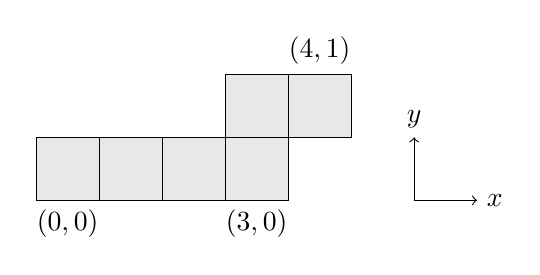
\begin{tikzpicture}[x=8mm,y=8mm]
\foreach \x/\y in {0/0,1/0,2/0,3/0,3/1,4/1}
 {\filldraw[fill=gray!18] (\x,\y) rectangle +(1,1);}
\node[below] at (.5,0) {$(0,0)$};
\node[below] at (3.5,0) {$(3,0)$};
\node[above] at (4.5,2) {$(4,1)$};
\draw[->] (6,0)--(7,0) node[right] {$x$};
\draw[->] (6,0)--(6,1) node[above] {$y$};
\end{tikzpicture}
\caption{The six cells of Snaky. A cell is indexed by the coordinates
of its lower left corner. Every integral translation and signed
coordinate permutation of this shape is an allowed target.}
\label{fig:target}
\end{figure}

\paragraph{Earlier results and methods.}
Sieben attributes the introduction of polyomino achievement games to
Frank Harary \cite[Section~1]{Sieben2004}. His account records
handicap-two strategies of Harary, Harborth and Seemann and the
nonexistence of a pairing defense for Snaky, and proves victory in
$41$ dimensions \cite[Section~4 and Proposition~4.1]{Sieben2004}.
Csernenszky, Martin and Pluh\'ar later gave a computer-free proof of
the nonexistence of a pairing defense
\cite[Theorem~10]{CsernenszkyMartinPluhar2011}.
This rules out a class of Breaker strategies, but does not by itself
give Maker a winning strategy.

Halupczok and Schlage-Puchta proved that Snaky wins in three
dimensions, loses on an $8\times8$ board, and has planar handicap
number at most one \cite[Theorem~1]{HSP2007}.
A handicap of one allows Maker two stones on the opening turn,
before Breaker's first reply.
Ito and Miyagawa also presented a handicap-one construction
\cite{ItoMiyagawa2007}.
Sieben subsequently gave a finite proof sequence for that handicap
and described the ordinary planar problem as undecided at the time
\cite[Section~1 and Appendix~B]{Sieben2008}.

Theorem~\ref{thm:main} treats the empty planar board without a handicap.
We give three complete constructions, with bounds of $21$, $25$, and
$35$ Maker moves. They share a
composition rule but retain different information and different openings.
The $21$-move certificate ends directly with no required Maker stones.
The $25$-move construction removes already-owned cells from each
Breaker-free region and uses required cells as placement anchors.
The $35$-move construction supplies four explicit conditional statements
at arbitrary positions and an opening that reaches one of them.
We keep these methods explicit because their content is not determined by the empty-board
move bounds alone.

Our method belongs to the proof-tree approach to weak achievement
studied by Sieben \cite[Sections~2--3]{Sieben2008}.
His finite situations and territory-intersection conditions encode
ways of combining continuations at Breaker's turn. Our conditional
positions are stated at Maker's turn, with a separate Breaker-turn
consequence for openings in which the pivot is already owned.
The formulation explicitly keeps track of arbitrary previous Maker
and Breaker ownership and counts actual future Maker moves.
We prove its soundness in Section~\ref{sec:templates}.
The perpendicular attacks discussed by Halupczok and Schlage-Puchta
\cite[Section~3]{HSP2007} also illuminate why a line of four Maker
stones can exert substantial pressure. Section~\ref{sec:geometry}
gives a separate, fully stated local result of this kind.

Shaik, Mayer-Eichberger, van de Pol and Saffidine studied bounded-depth
QBF encodings of finite Maker--Breaker games, including Snaky on a
$5\times5$ board \cite[Sections~2.1 and~6]{ShaikEtAl2023}.
Boucher and Villemaire study QBF encodings for finite strong achievement
games on ordinary and toroidal boards
\cite[Sections~2.2, 3.3--3.4, and~4]{BoucherVillemaire2025}.
Here the finite object is a proof of sufficient conditions for the
infinite weak game. Breaker is free to play outside every displayed
region, and the proof covers those replies without a board cutoff.

\paragraph{Proof overview.}
A conditional winning position is described by three finite data:
a set $A$ that Maker must own, a set $T$ that must contain no Breaker
cell, and a bound $h$ on further Maker moves. Starting with the six
immediate completions of $S$, we combine such conditions as follows.
Maker claims a chosen cell. The required cells of every child
condition then belong to Maker; moreover, the intersection of the
child envelopes belongs to Maker. Consequently one new Breaker cell
cannot lie in every child envelope, and at least one continuation
remains available.

Section~\ref{sec:certificate} specifies $728$ numbered conditions,
including the six bases, by exact integer coordinates and backward
references. The final one has $A=\varnothing$, an envelope of $251$
cells, and height $21$. Section~\ref{sec:strategy} turns the recursive
proof into one policy chosen before Breaker's play. The independent
four-in-a-row result follows in Section~\ref{sec:geometry}.
Section~\ref{sec:verification} distinguishes the mathematical induction,
exact data identities, and independent finite calculations.
Appendix~\ref{app:route25} proves the reduced-envelope construction and
its five-class opening. Appendix~\ref{app:route35} gives the complete
$35$-move construction, its unbounded opening, and its conditional tactics.
Appendix~\ref{app:formal} describes the finite reconstruction supplement.
Appendices~\ref{app:data}--\ref{app:data35}
print the three literal certificates, and Appendix~\ref{app:checker}
explains the standalone verification programs.

\section{Conditional winning positions}\label{sec:templates}\label{sec:calculus}

The purpose of this section is to justify a finite rule that remains
valid when Breaker may play anywhere on the infinite board.
At a finite position let $M,B\subset\Z^2$ be the finite disjoint
sets currently owned by Maker and Breaker. Their complete contents
are retained throughout the argument.

\begin{definition}\label{def:claim}
Let $A\subseteq T\subset\Z^2$ be finite and let $h\ge1$ be an integer.
The triple $(A,T,h)$ is a \emph{valid claim} if, at every position with
Maker to move and with
\[
 A\subseteq M,\qquad B\cap T=\varnothing,
\]
Maker has already completed a target or has a strategy that completes
one within $h$ further actual Maker moves. We call $A$ the required
set, $T$ the envelope, and $h$ the height.
\end{definition}

This definition imposes no restriction on additional Maker cells,
on Breaker cells outside $T$, or on how the position was reached.
In particular, it applies to arbitrary finite disjoint ownership,
without requiring a prescribed difference between $|M|$ and $|B|$.
Only the starting turn is specified.
A \emph{placement} is an affine map $F(x)=Rx+t$ with $R\in\G$ and
$t\in\Z^2$. A valid claim remains valid under the simultaneous
replacement of $A,T$ by $F(A),F(T)$, with the same height: the
bijection $F$ transports a legal strategy, preserves disjointness
and targets, and does not change the number of moves.

The use of finite sufficient conditions and alternative continuations
has a close antecedent in Sieben's proof trees and situations
\cite[Sections~2--3]{Sieben2008}. His situations consist of a Maker
core and a neighborhood without Breaker stones and are stated at
Breaker's turn; the proof trees use an empty intersection of
continuation territories. The rule below works with arbitrary finite
prior ownership and counts every actual fresh Maker claim. Its
quantitative form applies to all three constructions in this article.

\begin{lemma}[Combination rule]\label{lem:combination}\label{thm:composition}
Let $(A_i,T_i,h_i)$, $1\le i\le r$, be valid claims, where
$1\le r<\infty$, and let $p\in\Z^2$. Define
\begin{equation}\label{eq:combination}
 T=\{p\}\cup\bigcup_{i=1}^rT_i,
 \qquad
 A=\left(\bigcup_{i=1}^r A_i\ \cup\
             \bigcap_{i=1}^rT_i\right)\setminus\{p\},
 \qquad h=1+\max_i h_i.
\end{equation}
Then $(A,T,h)$ is valid. Also, at a position with Breaker to move,
if $A\cup\{p\}\subseteq M$ and $B\cap T=\varnothing$, then Maker
has already won or can win within $h-1$ further Maker moves.
\end{lemma}

\begin{proof}
Every $A_i$ is contained in $T_i$, so $A\subseteq T$.
Suppose first that Maker is to move, $A\subseteq M$,
$B\cap T=\varnothing$, and no target is yet complete.
Since $p\in T$, Breaker does not own $p$.
If $p$ is free, Maker claims it. If $p\in M$, Maker instead claims
any free cell. Such a cell exists because the board is infinite
and $M\cup B$ is finite. This replacement is one real move.
In both cases the resulting Maker set $M'$ contains
\begin{equation}\label{eq:intersection-owned}
 \bigcup_i A_i\ \cup\ \bigcap_iT_i
 \subseteq A\cup\{p\}\subseteq M'.
\end{equation}
If this move completes a target, stop immediately.
Otherwise let $b$ be the next legal Breaker cell. As $b\notin M'$,
\eqref{eq:intersection-owned} implies $b\notin\bigcap_iT_i$.
Choose an index $i$ with $b\notin T_i$.
The older Breaker cells also avoid $T_i$, since $T_i\subseteq T$.
Thus, at the next Maker turn,
\[
 A_i\subseteq M',\qquad (B\cup\{b\})\cap T_i=\varnothing.
\]
The child claim gives a win within $h_i$ more Maker moves.
Including the move already spent gives at most $1+h_i\le h$.

For the Breaker-turn assertion, the inclusions in
\eqref{eq:intersection-owned} already hold with $M$ in place of
$M'$. After Breaker's next move the same surviving child applies,
without spending the parent Maker move. Its bound is at most
$\max_i h_i=h-1$.
\end{proof}

The replacement move cannot invalidate this argument: it only adds
Maker ownership, and its actual ensuing Breaker reply is included
in the proof. It must not be omitted from the count.
A reply outside $T$ misses every child envelope, so distant play
requires no separate case analysis. The Breaker-turn assertion
also shows that $p$ need not have been Maker's most recent claim.

\begin{lemma}[Six bases]\label{lem:bases}
Write the points of $S$ in the order in \eqref{eq:target} as
$s_0,\ldots,s_5$. The claims
\begin{equation}\label{eq:bases}
 (A_j,T_j,h_j)=(S\setminus\{s_j\},S,1),
 \qquad 0\le j<6,
\end{equation}
are valid.
\end{lemma}

\begin{proof}
If Maker owns $s_j$, it already owns all of $S$.
Otherwise $s_j$ is free because Breaker owns none of $S$.
Claiming it completes the target in one move.
\end{proof}

Every application of Lemma~\ref{lem:combination} may use placed
versions of earlier claims. We will describe a finite collection of
such applications and calculate its last required set and height.
The semantic proof is already complete: once that required set is
empty, the final height bounds play from the empty board.

\section{The certificate and its final condition}\label{sec:certificate}

This section specifies the finite applications of the combination
rule. We use the word \emph{card} for a numbered claim in this
$21$-move certificate. Its numbering is independent of the $25$- and
$35$-move tables in Appendices~\ref{app:route25} and~\ref{app:route35}. Numbered references allow a previously proved claim to
be reused; an expression written in parentheses is simply an
additional, unnumbered application of the same rule.
The complete literal data are in Appendix~\ref{app:data}.

\subsection{Coordinates, placements, and expressions}

The coordinate alphabet is
\begin{center}
\texttt{0123456789ABCDEFG}.
\end{center}
A two-character word \texttt{XY} denotes the point $(x,y)$ whose
coordinates are the positions of \texttt{X} and \texttt{Y} in this
alphabet, counting from zero. For example, \texttt{88} means $(8,8)$,
\texttt{7A} means $(7,10)$, and \texttt{GG} means $(16,16)$.
The encoded pivots and translation vectors have nonnegative
coordinates; the sets produced after signed transformations may
contain negative coordinates.

A reference \texttt{j:sUV} means: take numbered card $j$, apply the
signed coordinate permutation $R_s$, and then translate by the point
encoded by \texttt{UV}. To compute $R_s$, negate the first coordinate
if the bit of weight $2$ is set, negate the second if the bit of
weight $4$ is set, and \emph{then} interchange the coordinates if the
bit of weight $1$ is set. The resulting maps are
\begin{equation}\label{eq:symmetries}
\begin{array}{c|cccc}
 s&0&1&2&3\\ \hline
 R_s(x,y)&(x,y)&(y,x)&(-x,y)&(y,-x)\\[2pt]
\end{array}
\quad
\begin{array}{c|cccc}
 s&4&5&6&7\\ \hline
 R_s(x,y)&(x,-y)&(-y,x)&(-x,-y)&(-y,-x).
\end{array}
\end{equation}
These are precisely the eight matrices in $\G$.
A bare reference \texttt{j} uses the identity placement.
References change neither the child's height nor the meaning of its
winning condition.

Every data line consists of its decimal card number $j$, a pivot
coordinate, and a nonempty ordered list of children. Each child is
either a reference or an expression of the form
\begin{center}
\texttt{(XY child child ...)}.
\end{center}
Such an expression combines its children at the pivot \texttt{XY}
using \eqref{eq:combination}. All coordinates inside parentheses
remain in the coordinate frame of the line. They are not offsets
from the enclosing pivot. When the entire card is later placed by
an affine map, that map transports every pivot and set in its proof.

Cards $0,\ldots,5$ are the six bases \eqref{eq:bases}.
The data specify cards $6,\ldots,727$ in order. Every numbered
reference in a line, including a reference inside parentheses,
is to a smaller card number. We evaluate innermost expressions
first, using \eqref{eq:combination} for the sets and height.
Consequently structural induction on each expression, followed by
induction on the line number, proves that every resulting card is
a valid claim. The finite calculation determines which sufficient
conditions this particular list produces.

\subsection{Two elementary cards}

The first two lines illustrate both the geometry and the encoding:
\begin{lstlisting}[basicstyle=\ttfamily\small]
6 14 4:100 5:101
7 05 6:001 6:405
\end{lstlisting}
For card $6$, the two bases are first transposed; the second is also
translated by $(0,1)$. Direct substitution gives
\begin{equation}\label{eq:first-card}
 A_6=\{(0,y):0\le y\le4\},\qquad
 T_6=A_6\cup\{(1,3),(1,4),(1,5)\},\qquad h_6=2.
\end{equation}
Claiming $(1,4)$ prepares two copies, completed respectively at
$(1,3)$ and $(1,5)$. Unless a copy is already complete, Breaker
can occupy at most one of these cells. Figure~\ref{fig:fork}
shows the two alternatives.

\begin{figure}[tb]
\centering
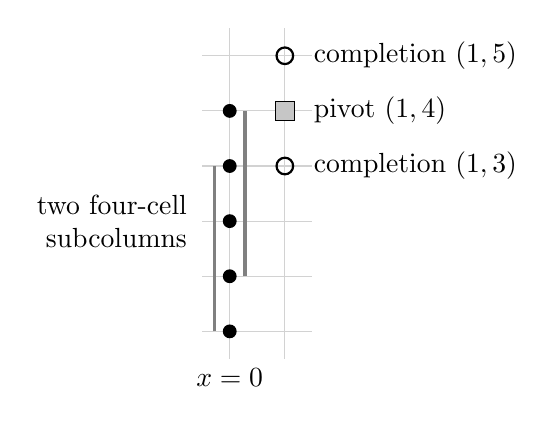
\begin{tikzpicture}[x=7mm,y=7mm]
\draw[gray!35,step=1] (-.5,-.5) grid (1.5,5.5);
\foreach \y in {0,1,2,3,4} {\fill (0,\y) circle (2.5pt);}
\draw[thick] (1,3) circle (3pt);
\draw[thick] (1,5) circle (3pt);
\filldraw[fill=gray!45] (.83,3.83) rectangle (1.17,4.17);
\node[right] at (1.35,3) {completion $(1,3)$};
\node[right] at (1.35,4) {pivot $(1,4)$};
\node[right] at (1.35,5) {completion $(1,5)$};
\node[below] at (0,-.5) {$x=0$};
\draw[very thick,gray] (-.28,0)--(-.28,3);
\draw[very thick,gray] (.28,1)--(.28,4);
\node[left,align=right] at (-.6,2) {two four-cell\\subcolumns};
\end{tikzpicture}
\caption{Card $6$: dots are required Maker cells, the square is the
next pivot, and circles mark the two possible completions. The
vertical guides indicate the two four-cell bodies. The envelope
contains no Breaker cell; any of its additional cells may already
belong to Maker.}
\label{fig:fork}
\end{figure}

For card $7$, the two copies of $A_6$ both occupy the column
$x=0$, $1\le y\le5$. Their additional envelope cells have heights
$4,5,6$ and $0,1,2$, respectively. These triples are disjoint, so
the intersection of the envelopes is precisely the common column.
Deleting the pivot $(0,5)$ therefore gives
\[
 \begin{split}
 A_7&=\{(0,y):1\le y\le4\},\qquad h_7=3,\\
 T_7&=\{(0,y):1\le y\le5\}
       \cup\{(1,y):y\in\{0,1,2,4,5,6\}\}.
 \end{split}
\]
The general certificate repeats this mechanism with longer
conditional continuations and cells that need not lie near the
current line of Maker stones.

\subsection{The final card}

\begin{proposition}\label{prop:certificate}
The data in Appendix~\ref{app:data} have exactly $722$ numbered
lines, with indices $6,\ldots,727$. Every line has a nonempty child
list, every reference uses an allowed placement of an earlier card,
and every parenthesized expression is a finite nonempty combination.
Together with the six bases, they produce $728$ valid claims.
Their heights are at most $21$, and the last card has
\begin{equation}\label{eq:final-card}
 p_{727}=(8,8),\qquad A_{727}=\varnothing,
 \qquad |T_{727}|=251,\qquad h_{727}=21.
\end{equation}
Moreover, $T_{727}\subseteq\{0,\ldots,16\}^2$.
\end{proposition}

\begin{proof}
The syntactic and set assertions are a finite calculation from
\eqref{eq:bases}, \eqref{eq:combination}, and
\eqref{eq:symmetries}, using the full displayed data.
The verifier in Appendix~\ref{app:checker} reconstructs every
numbered card. Its arrays initially contain the six bases.
Before line $j$ is processed, their entries at indices below $j$
are exactly the sets and heights specified by the preceding lines.
A reference retrieves an earlier entry and applies its stated
placement. Recursive evaluation applies \eqref{eq:combination}
at every parenthesized node and at the root of the line.
The nonempty-child and backward-reference tests make every union,
intersection, maximum, and lookup well-defined. This proves the
invariant for the next line and identifies the computed sets with
the mathematically defined ones. The final tests give
\eqref{eq:final-card}, maximum height $21$, and the intermediate
values in Table~\ref{tab:top}. The separate reconstruction
\nolinkurl{verification/supporting/independent_evaluator.py} also computes all
sets and heights and checks the successive intersections.
Validity then follows from Lemmas~\ref{lem:combination} and
\ref{lem:bases}, by the structural induction just described.
\end{proof}

For clarity, Table~\ref{tab:top} records how the final empty
requirement arises. The last line has $32$ placed children,
grouped by their six card numbers. Each placed required set is
exactly $\{(8,8)\}$. The last column is the number of cells other
than $(8,8)$ in the intersection of the envelopes from that group
and all preceding groups. The full placements occur in the last
line of the certificate.

\begin{table}[tb]
\centering
\begin{tabular}{rrrrrr}
\toprule
Card $j$ & $A_j$ & $|T_j|$ & $h_j$ & Placements & Remaining cells\\
\midrule
648 & $\{(4,5)\}$ & 87  & 15 & 4 & 35\\
708 & $\{(8,8)\}$ & 225 & 20 & 4 & 31\\
712 & $\{(5,5)\}$ & 96  & 15 & 8 & 21\\
713 & $\{(5,5)\}$ & 98  & 15 & 4 & 12\\
725 & $\{(7,7)\}$ & 167 & 20 & 8 & 4\\
726 & $\{(7,7)\}$ & 169 & 20 & 4 & 0\\
\bottomrule
\end{tabular}
\caption{The six groups of children in card $727$. All their
requirements become the pivot. Their common envelope has no other
cell, so the combination rule leaves an empty required set.}
\label{tab:top}
\end{table}

In particular, the intersection of all child envelopes is exactly
$\{(8,8)\}$: it contains that point because every child requirement
does, and the last table entry removes every other point.
The union of the child requirements is the same singleton.
Equation~\eqref{eq:combination} therefore gives $A_{727}=\varnothing$.
The maximum child height is $20$, giving the bound $21$.

The data also illustrate how play may leave an immediately adjacent
line. After Maker plays $(8,8)$ and Breaker replies $(7,8)$, the
placed child \texttt{708:100} is available. Its pivot is $(8,7)$.
If Breaker next takes $(8,6)$, the child \texttt{684:011} of card
$708$, still under the outer transposition, is available and has
pivot $(11,8)$. These are legal illustrative choices, not imposed
responses by Breaker. Every other reply is covered by the same
intersection rule.

\section{One strategy against every continuation}\label{sec:strategy}

We now turn the final card into a single strategy. Making its choices
definite also clarifies that the height counts actual Maker moves.

\begin{proof}[Proof of Theorem~\ref{thm:main}]
Fix an enumeration of $\Z^2$: order cells by increasing
$\max(|x|,|y|)$, then lexicographically within each finite level. Retain the printed order of the children in every
combination expression. These choices are fixed before any play.
Initially the active claim is card $727$ in its identity placement.
Its hypotheses hold on the empty board by
\eqref{eq:final-card}.

At an active combination with current placement $F$, claim its
placed pivot $F(p)$ if free. If Maker already owns $F(p)$, claim
the first free cell in the fixed enumeration instead. The invariant
of Definition~\ref{def:claim} guarantees that Breaker does not own
the pivot, and finiteness of ownership guarantees a free replacement.
Stop if a target is complete. Otherwise, after Breaker's next legal
reply, choose the first child in the printed list whose placed
envelope avoids that reply. Lemma~\ref{lem:combination} proves that
such a child exists and that all its requirements and its full
envelope satisfy the invariant, including the older Breaker cells.
For a referenced card whose reference placement is $G$, the new
placement is $F\circ G$; for an inline expression, retain $F$ and
use that expression.

At a placed base card, either the target is already present or its
one missing cell is free. In the latter case claim it and win.
Thus a nonterminal step spends one actual Maker move and passes,
after one actual Breaker reply, to a child of strictly smaller
height. The bases have height $1$. Starting at height $21$, this
procedure wins within $21$ Maker moves.

The active expression and placement are determined by the complete
history: replay the prescribed pivot or replacement choices and
the first-surviving-child choices from card $727$.
On a history inconsistent with an earlier prescribed Maker choice,
use the first free cell of the enumeration. Use the same fallback
on an already-won history if one chooses to continue it formally.
This defines a globally legal policy on all finite legal histories,
including histories not reached from the empty board under the
policy. No choice of the policy depends on future Breaker moves.
The preceding induction applies to every legal continuation from
the empty board and proves the theorem.
\end{proof}

Only replies before victory are used in this argument. If the first
win occurs on Maker move $m\le21$, there have been precisely $m-1$
Breaker moves. In particular, no reply after Maker's winning move
is assumed or required.

One can express the same quantifier order using a fixed endpoint.
Extend the policy beyond a completed target by the first-free-cell
rule. For every sequence of proposed Breaker cells whose first
$20$ entries are legal along this extended policy, the Maker set
immediately after move $21$ contains an allowed copy of $S$.
An earlier completed copy persists because ownership is permanent.
This formulation is $\exists\sigma\,\forall\beta$, with $\sigma$
chosen in the proof and $\beta$ the sequence of Breaker replies;
it makes no assumption about a twenty-first Breaker reply.
Stopping at the first target recovers the ordinary game.

\begin{corollary}[A finite board]\label{cor:finite-board}
Maker wins the weak Maker--Breaker game within $21$ actual Maker
claims on the initially empty $251$-cell board $T_{727}$, and also
on the initially empty $17\times17$ board $\{0,\ldots,16\}^2$.
In each game, Maker moves first, the players alternate claiming one
previously unclaimed cell, and the targets are the allowed copies
of $S$ contained in the board.
\end{corollary}

\begin{proof}
Evaluation of the literal certificate gives
\[
 T_{727}\subseteq\{0,\ldots,16\}^2,
\]
in addition to the endpoint data in \eqref{eq:final-card}.
Every placed child envelope is contained in its parent envelope,
and every pivot and base target lies in its own envelope. Thus all
prescribed pivots and base completions lie in $T_{727}$.
Use that strategy, replacing an already-owned pivot by the first
free cell in a fixed ordering of $T_{727}$. Before Maker claim
$m\le21$, at most $2(m-1)\le40$ cells have been occupied, so such
a replacement is always available on either board.

After a pivot or replacement claim, Maker owns every child
requirement and the intersection of the child envelopes. Every
legal Breaker reply therefore leaves a surviving child envelope;
nesting also keeps the older Breaker cells outside that envelope.
This includes replies outside $T_{727}$ on the square board.
The same height induction now gives victory within $21$ actual
Maker claims, counting each replacement. Play stops as soon as a
target is complete; no Breaker reply after victory is used.
\end{proof}

\section{Four stones in a row}\label{sec:geometry}

The certificate establishes the empty-board theorem without assuming
that nearby Breaker cells stay sparse. A separate local statement
explains some of the geometry behind its threats. The perpendicular
attack below is related to the four-in-a-row tactics of Halupczok
and Schlage-Puchta \cite[Section~3, pp.~13--15]{HSP2007}; their planar
row extensions also appear in Sections~4.4--4.6 of that paper.
We give a complete proof for the precise finite-neighborhood
hypothesis used here.

\begin{proposition}\label{prop:four-row}
Suppose it is Maker's turn at an arbitrary finite position, Maker
owns the four cells
\[
 \{(0,0),(1,0),(2,0),(3,0)\},
\]
and Breaker owns at most three cells in
\[
 Q=([-3,6]\times[-4,4])\cap\Z^2.
\]
Then Maker has already won or can force a win. Additional Maker
cells and arbitrary Breaker cells outside $Q$ are allowed.
\end{proposition}

Call a set \emph{clean} if it contains no Breaker cell.
Throughout this section, an instruction to claim an already-owned
Maker cell means to claim any free cell instead, unless a target
has already been completed. Such a replacement is a real move and
allows exactly one new Breaker reply. Extra Maker cells therefore
cause no difficulty in any of the arguments below.

When a move is said to force Breaker to a cell $q$, the precise
meaning is that $q$ completes an allowed target on Maker's next
move. If $q$ is already Maker's, the target is already complete.
Otherwise $q$ is free, and Breaker must claim it or allow that
immediate completion. Every forced continuation is considered only
when Maker has not already won or obtained this next-move win.

\subsection{A five-cell fork}

Suppose Maker owns the horizontal five
$\{(r,0),\ldots,(r+4,0)\}$. For an endpoint $e\in\{r,r+4\}$
and a sign $\varepsilon\in\{-1,1\}$, put
\begin{equation}\label{eq:horizontal-triple}
 H(e,\varepsilon)=
 \{(e-1,\varepsilon),(e,\varepsilon),(e+1,\varepsilon)\}.
\end{equation}
If this triple is clean at Maker's turn, claiming its middle cell
$(e,\varepsilon)$ creates two one-cell completions, at its other
two cells. The two targets use respectively the first and last
four-cell subrows of the five; they are reflected or translated
copies of $S$. Breaker can occupy at most one completion, so
Maker wins on the next move unless it has already won.
This is the horizontal version of Figure~\ref{fig:fork}.

The four triples in \eqref{eq:horizontal-triple} are pairwise
disjoint. Consequently, if Maker has just created the five and
at least two of these triples are clean \emph{before} Breaker's
response, at least one remains clean afterwards, and the fork
wins. The same assertion holds after interchanging the coordinates.
For a vertical five we use the notation
\[
 V(c,d)=\{(c,d-1),(c,d),(c,d+1)\},
\]
where $c\in\{-1,1\}$ and $d$ is an endpoint height.

\subsection{The perpendicular endpoint attack}

We first establish a local tactic at the right endpoint of a row.
Assume Maker owns the four cells
\[
 (-3,0),\quad(-2,0),\quad(-1,0),\quad(0,0),
\]
and the set
\begin{equation}\label{eq:endpoint-zone}
 Z=\{(x,y):x\in\{-1,0,1\},\ 1\le |y|\le4\}
\end{equation}
is clean. Other ownership is arbitrary.
Maker claims $(0,1)$, forcing $(1,1)$, and then $(0,-1)$,
forcing $(1,-1)$. Indeed, the original horizontal body with the
respective pair of cells above or below its endpoint is an allowed
Snaky. If Breaker declines either forced reply, Maker completes
that copy on its next turn.

After those two replies, Maker claims $(0,2)$. Denote the new
Breaker reply by $b$, and set
\[
E=\{(0,-2)\}\cup V(-1,-2)\cup V(-1,2).
\]
Figure~\ref{fig:endpoint-branches} separates the two possible
continuations after this reply.
If $b\notin E$, Maker claims $(0,-2)$. It now owns the vertical
five from height $-2$ to height $2$, and both $V(-1,-2)$ and
$V(-1,2)$ are clean before the ensuing Breaker reply. They are
disjoint, and neither of the two earlier forced Breaker cells is
in either triple. The five-cell fork therefore wins.

If $b\in E$, Maker instead claims $(0,3)$, creating the vertical
five from height $-1$ to height $3$. The triple $V(1,3)$ is clean.
The triple $V(-1,3)$ is also clean unless
\[
 b=(-1,2)\quad\hbox{or}\quad b=(-1,3).
\]
If both are clean, the same two-triple argument wins.
In either exceptional case there is instead an immediate
completion at $q=(-1,-1)$, because Maker already owns the other
five cells of
\begin{equation}\label{eq:perpendicular-copy}
 \{(0,3),(0,2),(0,1),(0,0),(-1,0),(-1,-1)\}
 =\{(-y,3-x):(x,y)\in S\}.
\end{equation}
The cell $q$ lies in the initially clean zone, and differs from
$b$ and from the two earlier forced replies. It is thus free
unless Maker already owns it, in which case the target is complete.
It also lies outside $V(1,3)=\{(1,2),(1,3),(1,4)\}$.
Breaker must either claim $q$, leaving that clean triple for the
five-cell fork, or leave $q$ as an immediate winning move.
This completes the endpoint tactic.

\begin{figure}[tb]
\centering
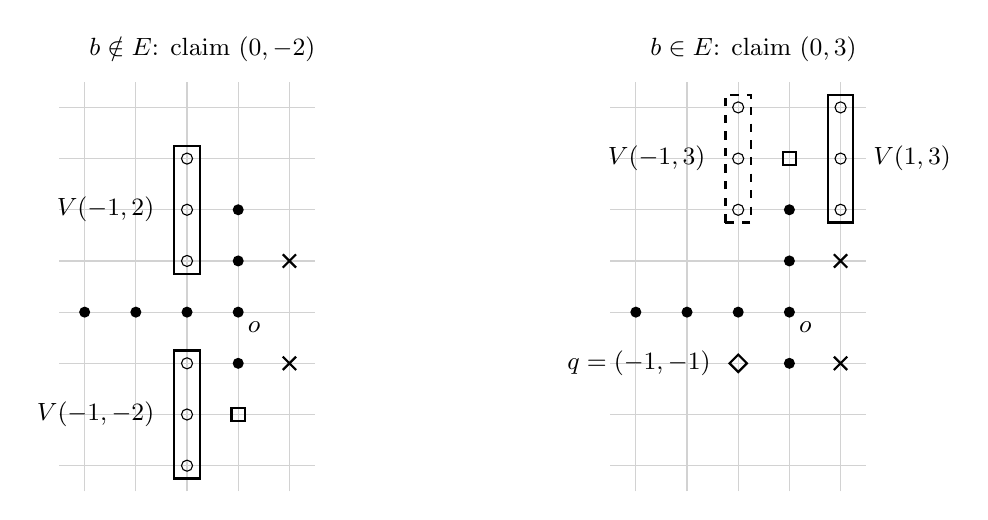
\begin{tikzpicture}[x=6.5mm,y=6.5mm,font=\small]
\foreach \shift in {0,7}{
 \begin{scope}[xshift=\shift cm]
 \draw[gray!35,step=1] (-3.5,-3.5) grid (1.5,4.5);
 \foreach \x/\y in {-3/0,-2/0,-1/0,0/0,0/-1,0/1,0/2}
  {\fill (\x,\y) circle (2pt);}
 \foreach \y in {-1,1}
  {\draw[thick] (.87,\y-.13)--(1.13,\y+.13)
                (.87,\y+.13)--(1.13,\y-.13);}
 \node[below right] at (0,0) {$o$};
 \end{scope}
}
\begin{scope}
\node[above] at (-.7,4.7) {$b\notin E$: claim $(0,-2)$};
\draw[thick] (-1.25,-3.25) rectangle (-.75,-.75);
\draw[thick] (-1.25,.75) rectangle (-.75,3.25);
\foreach \y in {-3,-2,-1,1,2,3}
 {\draw (-1,\y) circle (2pt);}
\draw[thick] (-.13,-2.13) rectangle (.13,-1.87);
\node[left] at (-1.45,-2) {$V(-1,-2)$};
\node[left] at (-1.45,2) {$V(-1,2)$};
\end{scope}
\begin{scope}[xshift=7cm]
\node[above] at (-.7,4.7) {$b\in E$: claim $(0,3)$};
\draw[thick,dashed] (-1.25,1.75) rectangle (-.75,4.25);
\draw[thick] (.75,1.75) rectangle (1.25,4.25);
\foreach \x in {-1,1}
 \foreach \y in {2,3,4}{\draw (\x,\y) circle (2pt);}
\draw[thick] (-.13,2.87) rectangle (.13,3.13);
\draw[thick] (-1,-.83)--(-.83,-1)--(-1,-1.17)--(-1.17,-1)--cycle;
\node[left] at (-1.45,3) {$V(-1,3)$};
\node[right] at (1.45,3) {$V(1,3)$};
\node[left] at (-1.35,-1) {$q=(-1,-1)$};
\end{scope}
\end{tikzpicture}
\caption{Alternative endpoint continuations after the reply $b$,
which is not drawn; here $o=(0,0)$. Dots show guaranteed Maker cells,
crosses the two earlier forced Breaker cells, and each square the
prescribed next claim.
Solid outlines enclose clean triples, whose cells may already be
Maker-owned. On the left, their union with the square is $E$.
On the right, the dashed triple is clean except when
$b=(-1,2)$ or $b=(-1,3)$; in those cases, claiming $(0,3)$
leaves the diamond $q$ as an immediate completion while $V(1,3)$ stays
clean. The panels are conditional alternatives, not consecutive moves.}
\label{fig:endpoint-branches}
\end{figure}

Every prescribed target or threat cell in this tactic lies in
$\{-3,-2,-1,0\}\times\{0\}$ or in $Z$.
Fresh replacement moves may be elsewhere on the board.
In particular, arbitrary Breaker moves outside the stated zone
are included in the preceding cases and cannot defeat the tactic.

\subsection{Proof of the four-in-a-row result}

\begin{proof}[Proof of Proposition~\ref{prop:four-row}]
Assume no target is already complete, and consider the two
extensions $(-1,0)$ and $(4,0)$ of the given row.

If both extensions belong to Breaker, there is at most one further
old Breaker cell in $Q$. The endpoint tactic has two possible
placements: at the left endpoint use $(x,y)\mapsto(-x,y)$, and
at the right endpoint use $(x,y)\mapsto(x+3,y)$.
Their off-row zones are respectively
\[
 \{-1,0,1\}\times\{-4,-3,-2,-1,1,2,3,4\}
 \quad\hbox{and}\quad
 \{2,3,4\}\times\{-4,-3,-2,-1,1,2,3,4\}.
\]
They are disjoint subsets of $Q$, and neither contains the two
row blockers. At least one zone is clean. The corresponding
endpoint tactic proves the result.

If exactly one extension belongs to Breaker, claim the other.
This produces a five in a row. The four endpoint triples are
pairwise disjoint and all lie in $Q$. The old row blocker meets
none of them, and at most two further old Breaker cells can meet
them. Thus at least two triples are clean before the new Breaker
response, and the five-cell fork wins.

It remains to consider the case that neither extension belongs
to Breaker. If one extension produces a five with at least two
clean endpoint triples, use it and finish as above. Suppose that
both choices fail this test. For extension to the left, the four
triples are $H(-1,\pm1),H(3,\pm1)$; for extension to the right,
they are $H(0,\pm1),H(4,\pm1)$.
Failure of either test requires at least three of its disjoint
triples to contain an old Breaker cell. Since at most three old
Breaker cells lie in $Q$, there are exactly three, and each must
meet a triple for both tests. A cell with this property lies on
level $-1$ or $1$ and has its first coordinate in $\{-1,0\}$
or in $\{3,4\}$. Moreover, their three combinations of
\emph{left or right cluster} and \emph{lower or upper level}
are distinct; otherwise fewer than three disjoint triples would
be met in one of the tests.

The reflections $(x,y)\mapsto(3-x,y)$ and
$(x,y)\mapsto(x,-y)$ preserve both the original four-cell row
and $Q$. They allow us to take the missing cluster-level
combination to be the lower right one. The three old Breaker
cells then have the form
\begin{equation}\label{eq:three-blockers}
 (l_-,-1),\quad(l_+,1),\quad(r,1),
 \qquad l_-,l_+\in\{-1,0\},\quad r\in\{3,4\}.
\end{equation}
No other old Breaker cell lies in $Q$.
Let $a$ count the true statements $l_-=0$, $l_+=0$, and $r=4$.

Suppose first that $a\ge2$. Claim $(-1,0)$.
The resulting five from $-1$ to $3$ has the clean triple
$H(3,-1)$. Unless Breaker meets it on its next move, Maker
uses that fork. Hence we may assume Breaker's new cell belongs
to $H(3,-1)=\{(2,-1),(3,-1),(4,-1)\}$.
Claim $(-2,0)$, which is free or already Maker's: neither an
old blocker nor that new cell can occupy it.
For the five from $-2$ to $2$, each of the following is a clean
endpoint triple when its indicated condition holds:
\[
\begin{array}{c|c}
\text{triple}&\text{condition}\\ \hline
H(-2,-1)&l_-=0\\
H(-2,1)&l_+=0\\
H(2,1)&r=4.
\end{array}
\]
They are pairwise disjoint and are all missed by the last
Breaker move. There are at least $a\ge2$ such triples before
the next response. The five-cell fork wins.

If $a\le1$, claim $(4,0)$ instead. Its clean lower-right triple
$H(4,-1)$ forces the next Breaker cell into
$\{(3,-1),(4,-1),(5,-1)\}$, or gives an immediate fork win.
Claim $(5,0)$, again free or already Maker's.
For the five from $1$ to $5$, the clean disjoint triples are
\[
\begin{array}{c|c}
\text{triple}&\text{condition}\\ \hline
H(1,-1)&l_-=-1\\
H(1,1)&l_+=-1\\
H(5,1)&r=3.
\end{array}
\]
At least $3-a\ge2$ conditions hold, and the most recent Breaker
cell meets none of these triples. The fork again wins.
All extension cells and triples in both cases lie in $Q$.
This exhausts the possibilities and proves the proposition.
\end{proof}

Proposition~\ref{prop:four-row} is a sufficient condition at an
arbitrary Maker turn. Its proof does not assume that the four
stones were obtained consecutively, and the $21$-move theorem
does not assume that its three-blocker hypothesis occurs during
play. The full certificate supplies the empty-board strategy.

\section{Finite verification and its scope}\label{sec:verification}

The three certificates describe finite applications of proved rules.
Their verification has three separate parts: the game-theoretic
soundness of those rules, the exact finite sets produced by the data,
and the identity of the distributed files. A checksum addresses only
the last part. The mathematical implication from a computed card to
every legal continuation is Lemma~\ref{lem:combination}, together with
the reduced-envelope bridge in Appendix~\ref{app:route25}.

\begin{center}
\begin{tabular}{lrrrr}
\toprule
Construction & Base cards & Numbered nonbase rows & References & Final bound\\
\midrule
$21$ moves & 6 & 722 & 4,089 & 21\\
$25$ moves & 6 & 2,010 & 5,862 & 25\\
$35$ moves & 6 & 610 & 1,837 & 35\\
\bottomrule
\end{tabular}
\end{center}
The reference count for the $21$-move construction includes occurrences
inside its $898$ inline combinations. It therefore has $1,620$
combination nodes altogether. The other two encodings have one
combination per nonbase row. Their row numbers and orientation codes
belong to three distinct tables.

\subsection{Exact reconstruction}

All calculations use finite sets of integer pairs. Each primary
program parses its literal data, checks the grammar and backward
references, applies the specified placements, and reconstructs every
required set, envelope, and height. A separate implementation for
each dialect independently parses and reconstructs the same data.
These programs are supplied with the complete editable source; no
strategy search, network connection, or undistributed game tree is
needed. Appendix~\ref{app:checker} gives the commands.

For the $21$-move certificate the reconstruction includes every inline
node, its enclosing coordinate frame, and the $32$ children of the
last card. It checks the endpoint, including containment of its
251-cell envelope in $\{0,\ldots,16\}^2$, the elementary cards, the
successive intersections in Table~\ref{tab:top}, and the nonlocal
continuation. There are $37,042$ local reply classes over all
combination nodes. For the $25$-move certificate it checks all
$2,010$ reduced compositions, their normalized full cards, the
required-size histogram, the five exceptional opening classes,
and the elementary and nonlocal examples. For the $35$-move
certificate it checks all $616$ templates, $26,703$ local reply
classes, the four terminal interfaces, and the longer tactical
identities in Appendix~\ref{app:route35}.

A local reply check uses the minimal Maker ownership required after
the pivot; additional Maker cells only remove possible legal replies.
One exterior case represents cells outside the parent envelope,
since every child envelope lies inside it. In the reduced encoding
this statement is applied after normalization. These finite checks
support the set calculations. Their coverage of arbitrary ownership
and the infinite board follows from the proved composition rule.
Likewise, tests of sample opening coordinates supplement the
symbolic whole-grid opening proof in Appendix~\ref{app:route35}.

The supplied test harnesses compare the full reconstructed cards,
not only terminal cardinalities. They also test rejection of
malformed or truncated inputs and execution with Python optimization.
Programs either use explicit exceptions for required checks or
refuse execution when assertions have been disabled. The harnesses
state their finite checks separately from the game-theoretic claims.

\subsection{Literal identities and formal coverage}

The literal data are printed in Appendices~\ref{app:data}--\ref{app:data35}.
Their literal SHA-256 identities are
\begin{lstlisting}[basicstyle=\ttfamily\scriptsize]
21: 3fa12d36a6d4dbb185e3f2808c8dfde13d85ee309afbca030d6ad17ae9fe3d04
25: 41cd04620af889771862dcceda7383afd99933ae03ddb0a566a00d742a8249b0
35: 16d077f0b64df70dd67fb6e9651636d42eaab0ce0f01f46180a57846e38fedc2
\end{lstlisting}
The middle file includes its initial newline and all $41$ index markers.
The source guide also records the normalized numeric serialization of
that table; it is a separate identity from the full literal. The
programs read these files as data and do not execute them as code.
Matching bytes do not replace reconstruction, and matching sets do
not replace the semantic induction or the move-count argument.

Appendix~\ref{app:formal} records the scope of the finite reconstruction
supplement for the $35$-move certificate. This supplement proves seven
finite reconstruction claims. It does not prove a complete winning
strategy, the $21$- or $25$-move construction, or the finite-board
corollary. The finite Python reconstructions do not themselves establish
a Lean theorem or kernel compilation. All three conventional proofs
are given independently of this supplement.

\bibliographystyle{plain}
\bibliography{references}
\appendix
\section{The reduced-envelope 25-move construction}\label{app:route25}

This construction records only those cells whose freedom from Breaker
is not already implied by Maker's required holdings.  It gives a second
finite strategy, with a different placement convention and a different
opening cover.  We first justify this representation and its exact
relationship to Section~\ref{sec:calculus}, then reconstruct the
certificate and explain its elementary and nonlocal attacks.

Throughout this appendix, a numbered \emph{$25$-card} belongs to the
family
\[
 \mathsf C^{25}_i=(P_i,E_i,h_i),\qquad 0\leq i\leq2015.
\]
The symbols $P_i,E_i,h_i$ in this appendix refer only to that family.
Its card numbers, placement codes, and local coordinates are independent
of the $21$- and $35$-move constructions.  In particular, their cards
with the same number need not have the same sets or meaning.

\subsection{Reduced requirements and their normalization}
\label{r25:semantics}

Let $P,E\subset\Z^2$ be finite and let $h\geq1$ be an integer.  A
\emph{valid reduced card} $(P,E,h)$ means the following: at every Maker turn with
finite disjoint ownership sets $M,B$, if
\begin{equation}\label{r25:condition}
 P\subseteq M,\qquad B\cap E=\varnothing,
\end{equation}
Maker has already won or can win within $h$ further actual Maker
claims.  We do not impose $P\subseteq E$, nor do we require $P$ and
$E$ to be disjoint.  Additional Maker cells and arbitrary Breaker
cells outside $E$ are allowed.  A signed permutation and translation
applied to both sets preserves validity and height, by the same
transport argument as for full cards.

The normalization
\begin{equation}\label{r25:normalization}
 (P,E,h)\longmapsto (A,T,h)=(P,P\cup E,h)
\end{equation}
preserves exactly the admissible positions.  Indeed, $P\subseteq M$
and $M\cap B=\varnothing$ already imply $B\cap P=\varnothing$;
under that assumption,
\[
 B\cap E=\varnothing
 \quad\Longleftrightarrow\quad
 B\cap(P\cup E)=\varnothing.
\]
Conversely, a full card $(A,T,h)$ with $A\subseteq T$ has the reduced
representative $(A,T\setminus A,h)$.  Normalizing this representative
returns $(A,T,h)$ exactly.  Normalizing an arbitrary $(P,E,h)$ and then
reducing replaces $E$ by $E\setminus P$; this changes no hypothesis
on a legal position.  Thus disjoint reduced sets are convenient
representatives, not an extra assumption in the semantics.

\begin{proposition}[Reduced composition]\label{r25:composition}
Let $(P_j,E_j,h_j)$, $1\leq j\leq m$, be valid reduced cards already
placed in one coordinate plane, where $1\leq m<\infty$.  Given an
attack cell $x$, put
\begin{equation}\label{r25:reduced-rule}
 \begin{aligned}
 U&=\bigcup_jP_j,& V&=\bigcup_jE_j,& I&=\bigcap_jE_j,\\
 H&=U\cup I,& P&=H\setminus\{x\},&
 E&=(V\setminus H)\cup\{x\},\qquad
 h=1+\max_jh_j.
 \end{aligned}
\end{equation}
Then $(P,E,h)$ is valid.  Its normalization is exactly the full card
obtained by Lemma~\ref{thm:composition} from the normalized children
$(P_j,P_j\cup E_j,h_j)$ at $x$; in particular, normalization changes
neither the required set nor the height.
\end{proposition}

\begin{proof}
We give the direct game argument, including the move that is needed
when the attack cell is already owned.  Suppose~\eqref{r25:condition}
holds for the parent and no target is complete.  Because $x\in E$,
Breaker does not own $x$.  If it is free, claim it.  Otherwise Maker
already owns it and claims any free cell instead; finite ownership on
$\Z^2$ guarantees that one exists.  This replacement consumes one
actual Maker claim, with its ensuing Breaker reply if play continues.
In either case the new Maker set $M'$ contains $H$, since it contains
$P$ and $x$.

Every older Breaker cell avoids every child envelope $E_j$.  To see
this without assuming $P_j\subseteq E_j$, note that the cells of $E_j$
outside $H$ lie in $E$, while its cells inside $H$ now belong to
Maker.  If the move has not won, the next legal Breaker cell $b$ is
outside $M'$, hence outside $I\subseteq H$.  Since the child list is
nonempty, some $E_j$ omits $b$.  At the next Maker turn this child
satisfies
\[
 P_j\subseteq U\subseteq M',\qquad
 (B\cup\{b\})\cap E_j=\varnothing.
\]
It wins in at most $h_j$ additional Maker claims.  The total is at most
$1+h_j\leq h$.  This also covers replies anywhere outside the finite
sets displayed in the construction.

For the asserted exact agreement, the pointwise identity is
\begin{equation}\label{r25:intersection-identity}
 U\cup\bigcap_j(P_j\cup E_j)
   =U\cup\bigcap_j E_j=H.
\end{equation}
For a point outside $U$, membership in $P_j\cup E_j$ is equivalent
to membership in $E_j$ for every $j$; points inside $U$ belong to both
sides.  This proves the identity without any containment or
disjointness assumption on the child sets.  Consequently the full
composition's required set is $H\setminus\{x\}=P$.  Its envelope is
\begin{align*}
 \{x\}\cup\bigcup_j(P_j\cup E_j)
   &=\{x\}\cup U\cup V\\
   &=\bigl(H\setminus\{x\}\bigr)
       \cup\bigl((V\setminus H)\cup\{x\}\bigr)=P\cup E.
\end{align*}
Here $I\subseteq V$, using the nonempty list.  Both height recursions
are $1+\max_jh_j$.
\end{proof}

The same argument has a Breaker-turn form.  If immediately before a
Breaker reply Maker owns $P\cup\{x\}$ and Breaker avoids $E$, then
after that reply a child applies within at most $\max_jh_j$ further
Maker claims.  The attack cell need not have been the latest Maker
claim.  This follows directly from ownership of $H$ and the older
Breaker avoidance proved above.

\subsection{Bases, anchors, and the decimal certificate}
\label{r25:decoder}

All attacks in the local coordinates of a $25$-card occur at
$o=(0,0)$.  Order the target cells as
\[
 (L_0,\ldots,L_5)=((0,0),(1,0),(2,0),(3,0),(3,1),(4,1)).
\]
Thus $S=\{L_0,\ldots,L_5\}$.  The six base cards are
\begin{equation}\label{r25:bases}
 P_i=(S\setminus\{L_i\})-L_i,
 \qquad E_i=\{o\},\qquad h_i=1,
 \qquad 0\leq i<6.
\end{equation}
If $o$ is already Maker's, the translated target $S-L_i$ is already
complete.  Otherwise $o$ is free and completes it in one move.
Their normalized envelopes are exactly $S-L_i$.

For a reference to card $j$, order its required set $P_j$
lexicographically, by the first coordinate and then the second,
starting with index zero.  Write a placement code $r$ uniquely as
$r=8k+d$, $0\leq d<8$, and let $a_{j,k}$ be the $k$th cell in that
order.  The code is defined only when $0\leq k<|P_j|$.  Set
\begin{equation}\label{r25:placement}
 \Phi_{j,r}(v)=R_d(v-a_{j,k}),
\end{equation}
where the signed permutations are given explicitly by
\begin{center}
\begin{tabular}{c*{4}{c}}
\toprule
$d$&$0$&$1$&$2$&$3$\\
\midrule
$R_d(x,y)$&$(x,y)$&$(y,x)$&$(-x,y)$&$(-y,x)$\\
\midrule
$d$&$4$&$5$&$6$&$7$\\
\midrule
$R_d(x,y)$&$(x,-y)$&$(y,-x)$&$(-x,-y)$&$(-y,-x)$\\
\bottomrule
\end{tabular}
\end{center}
Equivalently, swap first when $d$ is odd, then negate the first
coordinate for the bit of value $2$, and the second for the bit of
value $4$.  In particular codes $3$ and $5$ use the swap-first order;
they must not be interpreted using the $21$-card decoder.  Each map
in~\eqref{r25:placement} aligns one \emph{required} child cell with
the parent's attack $o$.  The anchor is taken from $P_j$, not $E_j$
or the normalized envelope.  A child placement inside a current
placement $F$ is $F\circ\Phi_{j,r}$.

The complete literal certificate, printed in Appendix~\ref{app:data25}
and supplied as \path{verification/supporting/route25/certificate.txt}, has $2010$ numeric lines
defining cards $6$ through $2015$ in order.  Blank lines have no
effect.  A marker \texttt{\# n} asserts that the next card number is
$n$ and creates no card.  There are $41$ such markers.  Every numeric
line consists of decimal blocks of exactly three digits.  At current
card $i$, read these blocks from left to right; a block with value $b$
decodes as follows:
\begin{equation}\label{r25:decimal}
\begin{array}{c|c|c}
\text{condition}&\text{referenced card }j&\text{placement code }r\\ \hline
0\leq b<240&\lfloor b/40\rfloor&b\bmod40\\
240\leq b<740&i-1-\lfloor(b-240)/100\rfloor&(b-240)\bmod100\\
740\leq b\leq999&10(b-740)+\lfloor c/100\rfloor&c\bmod100
\end{array}
\end{equation}
The last case consumes the next three-digit block as $c$ as well.
A missing second block is invalid.  Leading zeros are part of the
three-digit format.  Every resulting pair $(j,r)$ must satisfy
$0\leq j<i$ and the anchor range in~\eqref{r25:placement}, and each
numeric line must contain at least one pair.

For the decoded list $\mathcal L_i$ of card $i$, form the placed
children
\[
 (\Phi_{j,r}(P_j),\Phi_{j,r}(E_j),h_j),\qquad (j,r)\in\mathcal L_i,
\]
and apply~\eqref{r25:reduced-rule} at $x=o$ to define $P_i,E_i,h_i$.
Every placed required set contains $o$, because of its anchor.
The resulting $P_i$ and $E_i$ are disjoint, and $o\in E_i$.
These properties are consequences of the recurrence; the soundness
proof did not assume them.  All references are backward, so induction
from~\eqref{r25:bases} proves the validity of every card whose line
decodes.  No game-tree search or additional compatibility test is
needed: the union and intersection in the composition formula put
all necessary extra ownership into the parent's required set.

For example, \texttt{193233} decodes into $(4,33),(5,33)$.
The next line, \texttt{165272}, decodes at $i=7$ into $(4,5),(6,32)$.
At $i=2015$, \texttt{927400} is an extended term $(1874,0)$,
whereas \texttt{240} is the relative term $(2014,0)$.
Thus all three cases in~\eqref{r25:decimal} refer to the same
anchor placement rule after decoding.

\subsection{The first two composite cards}
\label{r25:elementary}

The first two rows exhibit both simultaneous finishes and transfer
after a forced block.  For card $6$, the two codes $33=8\cdot4+1$
use anchors $(1,0)\in P_4$ and $(-1,0)\in P_5$, respectively.
Their placed envelopes are the singletons $\{(0,-1)\}$ and
$\{(0,1)\}$.  Their placed required sets are
\[
 \{(-1,t):-4\leq t\leq-1\}\cup\{o\},\qquad
 \{(-1,t):-3\leq t\leq0\}\cup\{o\}.
\]
The intersection of the two singleton envelopes is empty.
Composition therefore gives exactly
\begin{equation}\label{r25:card6}
 P_6=\{(-1,t):-4\leq t\leq0\},\qquad
 E_6=\{(0,-1),o,(0,1)\},\qquad h_6=2.
\end{equation}
After the attack at $o$, the two one-hole copies have different
holes.  If neither is already complete, a single Breaker reply cannot
block both.  All five cells of the required column are outside $E_6$;
this is an explicit reason the reduced notation must allow
$P_6\not\subseteq E_6$.

For card $7$, code $5$ at card $4$ uses the first lexicographic anchor
$(-3,-1)$ and $R_5(x,y)=(y,-x)$.  Its placed required set and hole are
\[
 \{(0,-3),(0,-2),(0,-1),o,(1,-4)\},
 \qquad \{(1,-3)\}.
\]
Code $32=8\cdot4$ at card $6$ uses anchor $(-1,0)$ and is translation
by $(1,0)$.  Its placed required set is
$\{(0,t):-4\leq t\leq0\}$, its envelope is
$\{(1,-1),(1,0),(1,1)\}$, and its attack is $(1,0)$.
Again the two child envelopes are disjoint, giving
\begin{equation}\label{r25:card7}
 \begin{split}
 P_7&=\{(0,-4),(0,-3),(0,-2),(0,-1),(1,-4)\},\\
 E_7&=\{o,(1,-3),(1,-1),(1,0),(1,1)\},\qquad h_7=3.
 \end{split}
\end{equation}
After the attack at $o$, failure to block $(1,-3)$ lets Maker complete
the base child on the next move.  A block there leaves the translated
card $6$ available, whose next attack is $(1,0)$.  If one of these
attacks was already owned, the general card semantics either detects
an earlier target or charges the required fresh replacement.  The
ensuing reply is never skipped.  Figure~\ref{r25:elementary-figure}
displays the two configurations.

\begin{figure}[htbp]
\centering
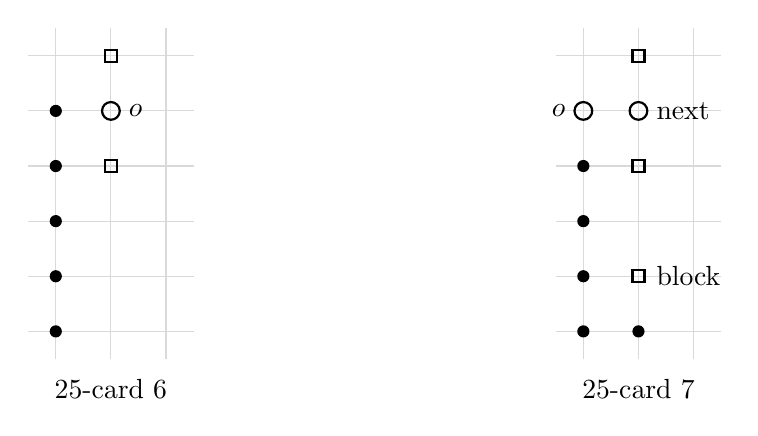
\begin{tikzpicture}[x=7mm,y=7mm]
 \begin{scope}
  \draw[gray!30,step=1] (-1.5,-4.5) grid (1.5,1.5);
  \foreach \y in {-4,-3,-2,-1,0}
    \fill (-1,\y) circle (2.2pt);
  \draw[thick] (0,0) circle (3.2pt);
  \node[right] at (0.15,0) {$o$};
  \foreach \y in {-1,1}
    \draw[thick] (-0.11,\y-0.11) rectangle (0.11,\y+0.11);
  \node[below] at (0,-4.7) {$25$-card $6$};
 \end{scope}
 \begin{scope}[xshift=6cm]
  \draw[gray!30,step=1] (-0.5,-4.5) grid (2.5,1.5);
  \foreach \y in {-4,-3,-2,-1}
    \fill (0,\y) circle (2.2pt);
  \fill (1,-4) circle (2.2pt);
  \draw[thick] (0,0) circle (3.2pt);
  \node[left] at (-0.15,0) {$o$};
  \draw[thick] (0.89,-3.11) rectangle (1.11,-2.89);
  \node[right] at (1.15,-3) {block};
  \draw[thick] (1,0) circle (3.2pt);
  \node[right] at (1.15,0) {next};
  \foreach \y in {-1,1}
    \draw[thick] (0.89,\y-0.11) rectangle (1.11,\y+0.11);
  \node[below] at (1,-4.7) {$25$-card $7$};
 \end{scope}
\end{tikzpicture}
\caption{The elementary reduced cards.  Solid disks are the required
Maker cells.  In card $6$, attacking the open disk $o$ gives the two
square-marked finishes.  In card $7$, the attack at $o$ threatens the
square $(1,-3)$; after that block, the open disk $(1,0)$ starts the
translated card $6$, with finishes at the other two squares.}
\label{r25:elementary-figure}
\end{figure}

\subsection{The complete finite reconstruction and its endpoint}
\label{r25:reconstruction}

We now apply the same recurrence to the entire literal, retaining
every row.  The supplied primary program
\path{verification/supporting/route25/verify_certificate.py} and independent
program \path{verification/supporting/route25/independent_certificate.py}
reconstruct its finite sets and heights.  Their checks include the
decimal grammar, every backward reference and anchor, the marker
numbers, the required number of rows, and the exact endpoint.
Malformed or truncated input is rejected; Appendix~\ref{app:checker}
gives the verification commands and their scope.  Their finite arithmetic
supports the set identities below; the reason these sets give a game
strategy is Proposition~\ref{r25:composition} and the induction just
proved, independently of either program.

The complete reconstruction has $2016$ cards and $5862$ placed child
terms.  The number of cards of each required-set size is
\begin{equation}\label{r25:histogram}
\begin{array}{c|rrrrrrrrrrr}
 |P_i|&0&1&2&3&4&5&6&7&8&9&10\\ \hline
 \text{number}&1&5&52&217&448&523&416&219&103&30&2.
\end{array}
\end{equation}
The last card can also be inspected through the much smaller
terminal table.  Its $28$ children comprise exactly the following
five groups in the printed order.  Each listed code has anchor index
$k=0$.  The last column gives the size of the intersection of all
placed reduced envelopes through the end of that row of the table.
\begin{table}[htbp]
\centering
\begin{tabular}{rcrrr}
\toprule
Child $j$&Codes $r$&$|E_j|$&$h_j$&Cumulative intersection\\
\midrule
$1874$&$0,1,2,5$&$292$&$24$&$184$\\
$1985$&$0,2,4,6$&$162$&$19$&$96$\\
$1996$&$0,1,2,5$&$117$&$15$&$49$\\
$1998$&$0,1,2,3,4,5,6,7$&$119$&$20$&$32$\\
$2014$&$0,1,2,3,4,5,6,7$&$76$&$14$&$0$\\
\bottomrule
\end{tabular}
\caption{All children of $25$-card $2015$.  The common reduced
envelope disappears after the last group.}
\label{r25:terminal-table}
\end{table}
The required sets of these five child cards are
\begin{equation}\label{r25:singleton-requirements}
 P_{1874}=P_{1985}=P_{1996}=\{(-1,0)\},\qquad
 P_{1998}=\{(0,1)\},\qquad P_{2014}=\{(1,0)\}.
\end{equation}
Every placed requirement is therefore $\{o\}$.  The table gives
$U=\{o\}$ and $I=\varnothing$, hence $H=\{o\}$ and
\begin{equation}\label{r25:terminal}
 P_{2015}=\varnothing,\qquad |E_{2015}|=389,\qquad h_{2015}=25.
\end{equation}
The last height is $1+24$, not a bound obtained by identifying this
certificate with either of the other two constructions.

For an explicit description of the final finite region, its section
at ordinate $y$ is empty when $|y|>11$; otherwise it is the set of
integer abscissae in the following table:
\begin{center}
\begin{tabular}{c|c@{\qquad}c|c}
\toprule
$|y|$&Abscissae $x$&$|y|$&Abscissae $x$\\
\midrule
$0$&$[-10,10]$&$6$&$[-9,9]$\\
$1$&$[-11,11]$&$7$&$[-7,7]$\\
$2$&$[-10,10]$&$8$&$[-6,6]$\\
$3$&$[-11,11]$&$9$&$[-6,6]$\\
$4$&$[-10,10]$&$10$&$[-5,5]$\\
$5$&$[-10,10]$&$11$&$\{-3,-1,1,3\}$\\
\bottomrule
\end{tabular}
\end{center}
Here intervals mean all integer points.  The row counts give
$21+2(23+21+23+21+21+19+15+13+13+11+4)=389$.

\begin{proposition}[The $25$-move strategy]\label{r25:bound}
There is one ordinary Maker policy on the infinite square board that,
from the empty position, completes a copy of $S$ within $25$ actual
fresh Maker claims against every legal Breaker continuation.  In the
fixed-endpoint formulation, after extending the policy by fresh moves
beyond an earlier win, the Maker set after its $25$th claim contains
a target whenever the first $24$ Breaker replies are legal along the
policy.
\end{proposition}

\begin{proof}
Induction using~\eqref{r25:bases} and
Proposition~\ref{r25:composition} proves the validity of all $2016$
cards.  Equation~\eqref{r25:terminal} therefore applies at the empty
position.  To fix one policy before the opponent's choices, fix an
enumeration of $\Z^2$ and the printed order of every child list.
Start with card $2015$ in its identity placement.  At a composite
card in placement $F$, take $F(o)$ if free, or the first free cell
of the enumeration if $F(o)$ is already owned.  Stop at a target.
If play continues, after the next legal Breaker reply choose the
first child $(j,r)$ whose placed reduced envelope avoids the current
Breaker set.  The composition proof guarantees its existence and its
required ownership.  Replace the active placement by
$F\circ\Phi_{j,r}$.  At a base, its hole is either already filled,
giving a target, or can be taken to finish one.

Each nonterminal descent consumes one actual fresh Maker claim,
including every replacement, and decreases the height.  No path from
height $25$ needs more than $25$ such claims.  As in
Section~\ref{sec:strategy}, the active card and placement are determined
by replaying the complete history.  On a history inconsistent with
the policy, or beyond a completed target, prescribe the first free
cell instead.  This makes the policy globally legal on finite legal
histories and fixes it independently of future replies.

If the first win is on claim $m\leq25$, exactly $m-1$ replies have
preceded it.  Thus only $24$ replies can be needed.  Under the extended
policy an earlier target persists, proving the fixed-endpoint
statement without any assumption on a $25$th Breaker reply.
\end{proof}

\subsection{Why only five first-reply classes need extra cards}
\label{r25:opening}

The final row can be understood geometrically as a cover of all first
Breaker replies.  After Maker takes $o$, each of the eight placements
$\Phi_{2014,d}$, $0\leq d<8$, has required set $\{o\}$.
Let $D$ be the intersection of their reduced envelopes.  The exact
finite calculation is
\begin{equation}\label{r25:opening-common}
 \begin{split}
 D={}&\{(\pm t,0),(0,\pm t):t=1,2,3\}\\
    &\ \cup\{(\pm1,\pm1)\}
      \cup\{(\pm2,\pm1),(\pm1,\pm2)\},
 \end{split}
\end{equation}
with independent signs.  It contains $24$ cells.  In particular
the sorted absolute coordinates, larger first, have exactly the five
values
\[
 (1,0),\quad(1,1),\quad(2,0),\quad(2,1),\quad(3,0).
\]
The set $D$ is invariant under all signed permutations: composing any
one of those permutations with the eight placements merely permutes
them.  Equation~\eqref{r25:opening-common} is a finite set identity,
so it covers unbounded first replies as well: for every $b\notin D$,
at least one of the eight envelopes omits $b$.  That placement of
card $2014$ is already available, giving at most $14$ further claims.

For the five remaining classes, the following placements omit the
listed first Breaker cell.  All use $k=0$ and have placed required
set $\{o\}$.
\begin{table}[htbp]
\centering
\begin{tabular}{cccrr}
\toprule
First Breaker cell&Child $j$&$d$&Next attack&Further bound $h_j$\\
\midrule
$(1,0)$&$1874$&$2$&$(-1,0)$&$24$\\
$(1,1)$&$1985$&$6$&$(-1,0)$&$19$\\
$(2,0)$&$1996$&$2$&$(-1,0)$&$15$\\
$(2,1)$&$1998$&$2$&$(0,-1)$&$20$\\
$(3,0)$&$1996$&$2$&$(-1,0)$&$15$\\
\bottomrule
\end{tabular}
\caption{The five exceptional opening classes for the $25$-move
construction.  Each bound begins at Maker's second turn.}
\label{r25:opening-table}
\end{table}
For example, the first placement is
$\Phi_{1874,2}(x,y)=(-x-1,y)$ because its anchor is $(-1,0)$;
the fourth is $\Phi_{1998,2}(x,y)=(-x,y-1)$ because its anchor is
$(0,1)$.  These formulas give the displayed attacks directly.
For an arbitrary reply in one of the five classes, choose a signed
permutation $Q$ taking its representative to that reply and use the
placement $Q\circ\Phi_{j,d}$.  It still requires only $o$, and its
envelope omits that reply.  Thus the table and the eight placements
of card $2014$ give a direct whole-board opening proof, with largest
total $1+24=25$.  The terminal row in
Table~\ref{r25:terminal-table} encodes a finite opening cover of this
kind using its specified $28$ placements.

\subsection{Two continuations that leave the initial line}
\label{r25:nonlocal}

We finish by following two actual children of card $1874$.  This
makes the composition of coordinate maps visible and shows why an
implementation must retain the complete envelopes.  Suppose Maker
has played $o$, Breaker has replied $(1,0)$, and Maker uses the first
row of Table~\ref{r25:opening-table} to attack $(-1,0)$.  The current
outer placement is
\[
 F(x,y)=\Phi_{1874,2}(x,y)=(-x-1,y),
 \qquad M=\{o,(-1,0)\},\qquad B=\{(1,0)\}
\]
before Breaker's next reply.  The two following continuations are
present in the literal row for card $1874$:
\begin{center}
\begin{tabular}{ccccc}
\toprule
Next reply&Child $j$&Code $r$&Anchor $a_{j,k}$&Next attack\\
\midrule
$(-1,-1)$&$1716$&$8$&$(-2,-1)$&$(-3,1)$\\
$(-2,0)$&$1752$&$3$&$(-2,0)$&$(-1,2)$\\
\bottomrule
\end{tabular}
\end{center}

For the first, the native required set is
$P_{1716}=\{(-3,-1),(-2,-1)\}$.  Since $8=8\cdot1+0$, the
lexicographic anchor is the second point, $(-2,-1)$, and
\[
 \Phi_{1716,8}(x,y)=(x+2,y+1),\qquad
 (F\circ\Phi_{1716,8})(x,y)=(-x-3,y+1).
\]
The transformed requirement is precisely $\{o,(-1,0)\}$.
The reduced envelope has $256$ cells and satisfies the exact check
\begin{equation}\label{r25:avoidance1}
 (F\circ\Phi_{1716,8})(E_{1716})
       \cap\{(1,0),(-1,-1)\}=\varnothing.
\end{equation}
Thus the old reply as well as the new reply is excluded, and the
transformed pivot is $(-3,1)$.  It is distinct from all four cells
then owned by either player.  Card $1716$ supplies a height-$23$
continuation after the first two Maker claims, consistent with the
total bound $25$.

For the second, $P_{1752}=\{(-2,0),(-2,1)\}$ and $r=3$ selects
the first anchor and the swap-first map $R_3(x,y)=(-y,x)$.  Hence
\[
 \Phi_{1752,3}(x,y)=(-y,x+2),\qquad
 (F\circ\Phi_{1752,3})(x,y)=(y-1,x+2).
\]
Its requirement is again exactly $\{o,(-1,0)\}$, while its
$93$-cell reduced envelope satisfies
\begin{equation}\label{r25:avoidance2}
 (F\circ\Phi_{1752,3})(E_{1752})
       \cap\{(1,0),(-2,0)\}=\varnothing.
\end{equation}
Its pivot $(-1,2)$ is free, and this child has height $15$.
Equations~\eqref{r25:avoidance1}--\eqref{r25:avoidance2} use the
complete reconstructed envelopes, not just the new pivot or the
required pair of Maker cells.

The two replies here are legal examples, not forced Breaker choices.
For either example the indicated child is usable; the globally fixed
first-surviving-child policy may select an earlier usable child in
the same row.  Other replies are covered by the full child list and
Proposition~\ref{r25:composition}.  Neither the game nor this
certificate restricts Maker's holdings to a connected shape: these
two attacks deliberately leave the initial horizontal pair.

\section{The 35-move construction and its conditional interfaces}
\label{app:route35}

This appendix gives a separate construction from six immediate-completion
cards and 610 further rows.  Besides an ordinary 35-move strategy, it
provides four conditional strategies with small required sets and
specified regions in which Breaker may already have played.  Those
conditional conclusions concern arbitrary prior ownership, so they do
not follow merely from a better bound for the empty board.
We retain both the complete opening and the transfer, opposite-tip, and
bent-shape continuations that explain how this certificate operates.

Throughout this appendix, \(A_i^{35},T_i^{35},h_i^{35}\) denote the required
set, envelope, and height of row \(i\) of the \emph{35-move certificate}.
These indices and the placement codes below are separate from those of
the 21- and 25-move constructions.  The meaning of a card is the
arbitrary-ownership meaning of Section~\ref{sec:calculus}: at any Maker
turn, finite disjoint sets \(M,B\) with
\(A_i^{35}\subseteq M\) and \(B\cap T_i^{35}=\varnothing\) permit a win
within \(h_i^{35}\) further actual Maker claims, unless a target is
already complete.  Additional ownership is allowed everywhere.

\subsection{The letter-and-offset certificate}
\label{r35:decoder}

Write the target points in the fixed order
\[
 s_0=(0,0),\quad s_1=(1,0),\quad s_2=(2,0),\quad
 s_3=(3,0),\quad s_4=(3,1),\quad s_5=(4,1),
 \qquad o=(0,0).
\]
The six initial cards are
\begin{equation}\label{r35:bases}
 T_i^{35}=S-s_i,\qquad
 A_i^{35}=T_i^{35}\setminus\{o\},\qquad h_i^{35}=1
 \quad(0\le i\le5).
\end{equation}
They are valid by immediate completion.  If the missing point is already
Maker-owned, the target has already been obtained.

For \(i=6,\ldots,615\), the literal row consists of \(i\) followed by a
nonempty list of placement terms.  A term \texttt{kLuv} contains an
earlier decimal row index \(k<i\), one letter \(L\), and two individual
decimal digits \(u,v\).  Its placement is
\begin{equation}\label{r35:placement}
 F_{Luv}(x,y)=R_L(x,y)+(u-4,v-4),
\end{equation}
with the eight maps specified by
\begin{center}
\small
\begin{tabular}{c|cccc}
\(L\)&a&b&c&d\\ \hline
\(R_L(x,y)\)&\((x,y)\)&\((y,x)\)&\((x,-y)\)&\((-y,x)\)\\[3pt]
\(L\)&e&f&g&h\\ \hline
\(R_L(x,y)\)&\((-x,y)\)&\((y,-x)\)&\((-x,-y)\)&\((-y,-x)\)
\end{tabular}
\end{center}
Thus \texttt{614b43} means \((x,y)\mapsto(y,x-1)\), including its
translation; it is not one of the decimal orientation codes used in the
other two certificates.

If the terms of row \(i\) are \((k_j,L_ju_jv_j)\), put
\(C_j=F_{L_ju_jv_j}(A_{k_j}^{35})\) and
\(D_j=F_{L_ju_jv_j}(T_{k_j}^{35})\).  Define
\begin{equation}\label{r35:recursion}
 \begin{split}
 T_i^{35}&=\{o\}\cup\bigcup_j D_j,\\
 A_i^{35}&=\left(\bigcup_j C_j\ \cup\ \bigcap_jD_j\right)
             \setminus\{o\},\\
 h_i^{35}&=1+\max_j h_{k_j}^{35}.
 \end{split}
\end{equation}
Lemma~\ref{thm:composition} and induction on \(i\) prove every card
defined in this way.  The inductive argument is valid for every
syntactically correct list of backward references; the particular list
determines the useful required sets and envelopes.

For clarity, the complete finite substitution can be performed as
follows.  Initialize the six triples by \eqref{r35:bases}.  Read each
remaining row in increasing order, reject an empty list or a reference
outside \(0,\ldots,i-1\), decode each affine map by
\eqref{r35:placement}, and apply it to both stored sets.  Take the union
and intersection in \eqref{r35:recursion}, store the resulting triple,
and proceed to the next row.  All coordinates are integers and all sets
are finite.  At the end of each iteration the stored triples are
exactly the triples defined by the displayed equations, which is the
loop invariant justifying the reconstruction.

The complete 610-row literal is printed in Appendix~\ref{app:data35}
and supplied as \nolinkurl{verification/supporting/prior-35/certificate.txt}; it has
one row per line, including the final newline.  The primary and two
independent reconstructions are described in Appendix~\ref{app:checker}.
They use, respectively,
integer matrices and ordinary set operations, quarter turns and
incidence masks, and signed coordinate lookups with cellwise membership
tests.  Thus no search procedure or undisclosed strategy tree is needed
to recover the certificate.

\subsection{The first two compositions: five cells in a row}
\label{r35:elementary}

The first two nonbase rows are
\[
 \texttt{6 0a03},\qquad \texttt{7 4a34 6a54}.
\]
Set
\[
 L_- = \{-4,-3,-2,-1\}\times\{-1\},\qquad
 L_+ = \{-3,-2,-1,0\}\times\{-1\}.
\]
Row 6 has
\[
 T_6^{35}=S+(-4,-1)=L_-\cup\{(-1,0),o\},\qquad
 A_6^{35}=L_-\cup\{(-1,0)\},\qquad h_6^{35}=2.
\]
The height is the recursively assigned upper bound: after claiming its
pivot, Maker has in fact completed this target immediately.

The two placed children in row 7 have
\begin{equation}\label{r35:elementary-children}
\begin{array}{c|c|c}
\text{term}&\text{required set}&\text{envelope}\\ \hline
\texttt{4a34}&L_-\cup\{o\}&L_-\cup\{(-1,0),o\}\\
\texttt{6a54}&L_+\cup\{o\}&L_+\cup\{o,(1,0)\}.
\end{array}
\end{equation}
Their common envelope is
\((\{-3,-2,-1\}\times\{-1\})\cup\{o\}\), already contained in the
union of their required sets.  Consequently
\[
 A_7^{35}=\{-4,-3,-2,-1,0\}\times\{-1\},\qquad
 T_7^{35}=A_7^{35}\cup\{(-1,0),o,(1,0)\},\qquad h_7^{35}=3.
\]
After Maker owns the five lower cells and the pivot \(o\), either
\((-1,0)\) or \((1,0)\) completes one of the two displayed copies.
Both lie in the parent envelope, so neither is occupied by an earlier
Breaker stone.  If neither target is already complete, Breaker can
claim at most one of these two cells.  This is the elementary double
threat that the longer compositions reuse.  Its direct two-claim bound
is sharper than the stored height 3; the certificate deliberately uses
the uniform recursion \eqref{r35:recursion}.

\subsection{Four conditional outputs}
\label{r35:outputs}

The following finite identities supply the opening.  A set in the last
column is wholly disjoint from the envelope; it is not asserted to be
the entire complement of that envelope.

\begin{proposition}\label{r35:conditional}
The 35-move certificate has 616 cards, including its six base cards,
and 1,837 placement terms.  Every card satisfies
\(A_i^{35}\subsetneq T_i^{35}\),
\(o\in T_i^{35}\setminus A_i^{35}\), and \(h_i^{35}\le34\).
Four of its conditional interfaces are
\begin{equation}\label{r35:conditional-table}
\begin{array}{c|c|r|r|l}
 i&A_i^{35}&|T_i^{35}|&h_i^{35}&\text{region disjoint from }T_i^{35}\\ \hline
 557&\{(-1,0)\}&118&19&\{(x,y):x\le-3,\ y\le-2\}\\
 595&\{(-1,0)\}&222&27&\{(x,y):x=-2,\ y\le-2\}\\
 603&\{(-1,0)\}&275&27&\{(x,y):x\le-3,\ y=0\}\\
 615&\{(1,0)\}&686&34&\{(1,-1)\}.
\end{array}
\end{equation}
Each row applies at any Maker turn with its required point owned and
its entire envelope free of Breaker, regardless of all other ownership.
For row 615 there is also a Breaker-turn conclusion: if Maker owns
\(\{o,(1,0)\}\) and Breaker avoids \(T_{615}^{35}\), then after any
legal next reply Maker wins within 33 further claims, unless already
victorious.
\end{proposition}

\begin{proof}
The finite identities follow by the substitutions
\eqref{r35:bases}--\eqref{r35:recursion}.  The delivered reconstructions
check every row index, every placement and backward reference, the full
sets and heights, and the four outputs in
\eqref{r35:conditional-table}.  An omitted infinite region is checked
by testing its defining predicate at \emph{every} point of the finite
envelope.  For example, the first check verifies
\(x>-3\) or \(y>-2\) for every \((x,y)\in T_{557}^{35}\); this proves
disjointness from the whole infinite region, without sampling it.

For each composed card the reconstruction also verifies
\(C_j\subseteq A_i^{35}\cup\{o\}\) and \(D_j\subseteq T_i^{35}\).
It checks each possibly legal local reply in
\(T_i^{35}\setminus(A_i^{35}\cup\{o\})\), and one extra class
representing all cells outside \(T_i^{35}\).  There are 26,703 such classes in total over
the 610 composed rows.  In each class some child envelope is missed.
The exterior class is exact because every child envelope is contained
in the parent envelope.  Extra Maker ownership can only remove legal
reply cells, and earlier Breaker ownership is excluded by the envelope
hypothesis.  These checks establish the stated finite identities; the
game-theoretic conclusion is the induction using
Lemma~\ref{thm:composition}, not an inference from the number of tests.
Its Breaker-turn assertion gives the final claim, since
\(h_{615}^{35}-1=33\).
\end{proof}

\subsection{The complete ordinary opening}
\label{r35:opening}

\begin{theorem}\label{r35:theorem}
There is one ordinary Maker policy on the initially empty infinite
square board that completes an allowed copy of \(S\) within 35 actual
Maker claims against every legal Breaker play.  Equivalently, after
extending a won position by fresh moves if necessary, its 35th Maker
set contains a target whenever the first 34 Breaker replies are legal.
No 35th Breaker reply is required.
\end{theorem}

\begin{proof}
Maker first claims the actual origin.  Write \(q_*\ne o\) for Breaker's
first cell, and let \(0\le a\le b\) be the sorted absolute values of its
two coordinates.  Since the cell differs from the origin, \(b\ge1\).
We first handle all unbounded distant replies, and then the eight
adjacent or diagonal replies.

Suppose \(b\ge2\).  In local coordinates put \(p=(-1,0)\), and choose
\begin{equation}\label{r35:distant-choice}
 (i,d)=
 \begin{cases}
 (557,(-a,-b)),&a\ge2,\\
 (595,(-1,-b)),&a=1,\\
 (603,(-b,0)),&a=0.
 \end{cases}
\end{equation}
In each case \(d\) and \(q_*\) have the same sorted absolute
coordinates, so there is a signed permutation \(R\in\mathcal G\) with
\(Rd=q_*\).  Use the affine map
\begin{equation}\label{r35:opening-map}
 F(z)=R(z-p).
\end{equation}
It sends the required cell \(p\) to Maker's first cell, and the local
Breaker cell \(p+d\) to \(q_*\).  In the three respective cases,
\[
 p+d=(-a-1,-b),\qquad (-2,-b),\qquad (-b-1,0).
\]
The first has \(x\le-3,y\le-2\), the second has \(x=-2,y\le-2\), and
the third has \(x\le-3,y=0\).  Thus it lies in the corresponding
omitted region in \eqref{r35:conditional-table}.  At Maker's second
turn, \(F(A_i^{35})\) is owned and \(F(T_i^{35})\) contains no Breaker
cell.  The placed conditional card applies, giving totals at most
\(1+19=20\), \(1+27=28\), and \(1+27=28\), respectively.  The
argument used no upper bound on \(a\) or \(b\).

It remains to treat \(b=1\).  Put
\[
 q=(1,-1),\qquad P=\{o,(1,0)\},\qquad
 p=\begin{cases}(1,0),&a=0,\\o,&a=1.\end{cases}
\]
For the coordinate-adjacent reply, \(q-p=(0,-1)\); for the diagonal
reply, \(q-p=(1,-1)\).  In either case choose \(R\in\mathcal G\) with
\(R(q-p)=q_*\), and again use \eqref{r35:opening-map}.  Then
\(F(p)=o\) and \(F(q)=q_*\).  Maker's second move claims the other
cell of \(F(P)\).  It is fresh: the two cells of \(P\) differ, and
\(q\notin P\).  Immediately after this move,
\[
 M=F(P)=F(A_{615}^{35}\cup\{o\}),\qquad
 B=\{F(q)\},\qquad B\cap F(T_{615}^{35})=\varnothing.
\]
The two Maker cells have been obtained with the actual first Breaker
reply between them.  In the adjacent case the local pivot \(o\) was
played second; in the diagonal case it was played first.  This order
does not matter to the state-based Breaker-turn assertion of
Proposition~\ref{r35:conditional}.

It is now Breaker's second turn.  Every legal reply misses at least
one child envelope of the placed row 615, with that child's required
set already owned.  The child wins within at most 33 further Maker
claims.  Thus the total in the near case is
\[
 2+33=35.
\]
Figure~\ref{r35:near-figure} records both possible orders of the domino.

\begin{figure}[tb]
\centering
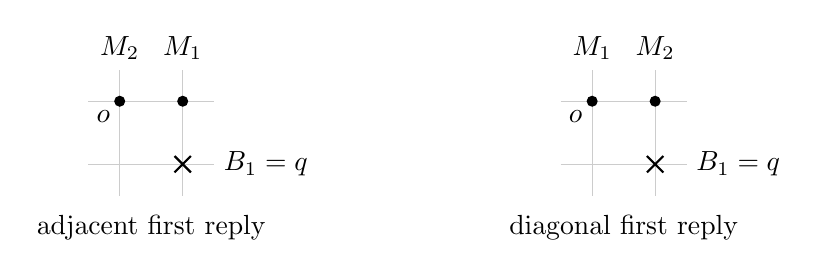
\begin{tikzpicture}[x=8mm,y=8mm]
\begin{scope}
\draw[gray!40,step=1] (-.5,-1.5) grid (1.5,.5);
\fill (0,0) circle (2pt); \fill (1,0) circle (2pt);
\node[above] at (0,.5) {$M_2$}; \node[above] at (1,.5) {$M_1$};
\node[below left] at (0,0) {$o$};
\draw[thick] (.87,-1.13)--(1.13,-.87) (.87,-.87)--(1.13,-1.13);
\node[right] at (1.5,-1) {$B_1=q$};
\node at (.5,-2) {adjacent first reply};
\end{scope}
\begin{scope}[xshift=6cm]
\draw[gray!40,step=1] (-.5,-1.5) grid (1.5,.5);
\fill (0,0) circle (2pt); \fill (1,0) circle (2pt);
\node[above] at (0,.5) {$M_1$}; \node[above] at (1,.5) {$M_2$};
\node[below left] at (0,0) {$o$};
\draw[thick] (.87,-1.13)--(1.13,-.87) (.87,-.87)--(1.13,-1.13);
\node[right] at (1.5,-1) {$B_1=q$};
\node at (.5,-2) {diagonal first reply};
\end{scope}
\end{tikzpicture}
\caption{Local coordinates immediately after Maker's second claim and
before Breaker's second reply.  Dots are Maker's domino \(P\), the
cross is the existing Breaker cell \(q\), and subscripts show the order
of the actual moves.  Row 615 controls the next reply in both cases.}
\label{r35:near-figure}
\end{figure}

Fix the choices before play: order the eight signed permutations and
the terms in every row, and fix an enumeration of \(\mathbb Z^2\).
Use the first admissible opening matrix and the first child envelope
missed by the latest reply.  Compose each child map with the current
affine frame.  If its pivot is already Maker-owned and no target is
complete, claim the first genuinely free cell in the enumeration;
that replacement and the following legal reply are charged in the
height recursion.  Every child has smaller index, so the recursion
terminates within the stated height.  On histories inconsistent with
earlier prescriptions, use the first free cell.  This gives one total
fresh policy, with the same early-stopping and extension conventions as
Section~\ref{sec:strategy}.  An extended 35-claim play contains only
34 intervening Breaker replies, proving the precise endpoint.
\end{proof}

\subsection{Transferring a four-cell attack to a new pair}
\label{r35:transfer}

We now examine the longer tactics inside the certificate.  They explain
how a small required set can support a continuation even after several
forced parries.  The conditions always concern the entire envelope;
the visible stones alone do not license a card.

Put \(V=\{-1\}\times\{-4,-3,-2,-1\}\).  The relevant literal rows and
reconstructed outputs are
\[
 \texttt{588 3b33 586a45},\qquad
 \texttt{589 4b43 588a45},
\]
\begin{equation}\label{r35:transfer-data}
\begin{array}{c|c|r|r}
i&A_i^{35}&|T_i^{35}|&h_i^{35}\\ \hline
586&\{(0,-2),(0,-1)\}&198&26\\
588&(V\setminus\{(-1,-1)\})\cup\{(0,-1)\}&202&27\\
589&V&204&28.
\end{array}
\end{equation}
Their envelopes satisfy the more informative identities
\begin{equation}\label{r35:transfer-envelopes}
\begin{split}
T_{588}^{35}&=(T_{586}^{35}+(0,1))\cup V,\\
T_{589}^{35}&=(T_{586}^{35}+(0,2))
 \cup (\{-1\}\times\{-4,-3,-2,-1,0\})\cup\{(0,-1)\}.
\end{split}
\end{equation}
In particular, each smaller continuation envelope is contained in the
envelope under which the tactic starts.

For an explicit description of these envelopes, Table~\ref{r35:fibers}
gives every vertical fiber of \(T_{586}^{35}\).  In this table
\([a,b]_{\mathbb Z}\) means every integer from \(a\) to \(b\), and
unlisted fibers are empty.  Together with
\eqref{r35:transfer-envelopes}, it specifies all three complete
envelopes, including cells far from the initial column.
\begin{table}[tb]
\centering\small
\begin{tabular}{c|l@{\qquad}c|l@{\qquad}c|l}
\(x\)&\(\{y:(x,y)\in T_{586}^{35}\}\)&
\(x\)&\(\{y:(x,y)\in T_{586}^{35}\}\)&
\(x\)&\(\{y:(x,y)\in T_{586}^{35}\}\)\\ \hline
\(-7\)&\([3,4]_{\mathbb Z}\cup\{6\}\)&0&\([-2,9]_{\mathbb Z}\)&7&\([-5,5]_{\mathbb Z}\)\\
\(-6\)&\(\{1\}\cup[3,6]_{\mathbb Z}\)&1&\([-6,9]_{\mathbb Z}\)&8&\([-2,4]_{\mathbb Z}\)\\
\(-5\)&\([-1,9]_{\mathbb Z}\)&2&\([-7,9]_{\mathbb Z}\)&9&\([-2,4]_{\mathbb Z}\)\\
\(-4\)&\([-1,8]_{\mathbb Z}\)&3&\([-6,9]_{\mathbb Z}\)&10&\([-2,0]_{\mathbb Z}\)\\
\(-3\)&\([-1,11]_{\mathbb Z}\)&4&\([-7,7]_{\mathbb Z}\)&11&\(\{-2,0\}\)\\
\(-2\)&\([-2,10]_{\mathbb Z}\)&5&\([-5,6]_{\mathbb Z}\)&&\\
\(-1\)&\([-1,11]_{\mathbb Z}\)&6&\([-5,6]_{\mathbb Z}\)&&
\end{tabular}
\caption{The complete 198-cell envelope of row 586.  The translated
envelopes governing the two forced parries and the transferred pair
follow from \eqref{r35:transfer-envelopes}.}
\label{r35:fibers}
\end{table}

Suppose \(V\subseteq M\) and \(B\cap T_{589}^{35}=\varnothing\) at a
Maker turn.  Claim \(o\) (or make the charged fresh replacement if it
is already owned).  The set
\[
 Q_1=V\cup\{o,(0,-1)\}
\]
is the target in the placed base card \texttt{4b43}.  Its only possibly
missing Maker cell is \((0,-1)\).  If this point is already owned,
Maker has won.  Otherwise it is free, because it lies in the parent
envelope.  A Breaker reply other than \((0,-1)\) leaves that immediate
completion available, so any defense avoiding this win must claim
\((0,-1)\).

The other child \texttt{588a45} uses the map \(z\mapsto z+(0,1)\).
Its required set is
\[
 (\{-1\}\times\{-3,-2,-1\})\cup\{o\},
\]
which is contained in the Maker set.  Its envelope
\(T_{588}^{35}+(0,1)\) is a subset of \(T_{589}^{35}\) and omits
\((0,-1)\).  All Breaker cells, including that first parry, therefore
avoid it.  Claim its pivot \((0,1)\), with the same charged-replacement
convention if necessary.  Now
\[
 Q_2=\{(-1,-3),(-1,-2),(-1,-1),(-1,0),o,(0,1)\}
\]
is complete except possibly at \((-1,0)\).  It is another allowed
target: \(Q_1=R_b(S)+(-1,-4)\) and
\(Q_2=R_b(S)+(-1,-3)\).  Thus, unless Maker has already won or can
complete \(Q_2\) on the next move, Breaker must parry at \((-1,0)\).

After these two parries, the continuation \texttt{586a45} of the
translated row 588 is row 586 translated by \((0,2)\).  Its required
set is exactly \(\{o,(0,1)\}\), now owned.  Its envelope
\[
 D=T_{586}^{35}+(0,2)
\]
lies in the original envelope and contains neither parry:
\((0,-1)\notin D\) and \((-1,0)\notin D\).  These omissions follow
directly from the fibers \(x=0\) and \(x=-1\) in
Table~\ref{r35:fibers}.  The envelope of the preceding row-588
continuation likewise omits the first parry by
\eqref{r35:transfer-envelopes}.  Row 586 therefore applies at the next
Maker turn, with pivot \((0,2)\) and bound 26.  The two earlier claims
and their forced replies have transferred the attack from the original
column to a new vertical pair, at total cost at most
\(1+1+26=28\) Maker claims.

This argument preserves every earlier Breaker restriction: all earlier
Breaker cells lie outside the original envelope and hence outside every
continuation envelope.  Extra Maker cells may complete a target early
or occupy one of the prescribed pivots; in the latter case a genuinely
fresh replacement uses the same charged turn.  No assumption that the
displayed stones are the only owned stones is needed.

\subsection{Opposite-tip continuations from four in a row}
\label{r35:opposite}

Row 612 consists exactly of
\[
 \texttt{612 589b55 589h03}.
\]
Writing
\[
 W=\{-3,-2,-1,0\}\times\{0\},\qquad
 G_+(x,y)=(y+1,x+1),\quad
 G_-(x,y)=(-y-4,-x-1),
\]
the two placed requirements are both \(W\), and their envelopes obey
\begin{equation}\label{r35:opposite-intersection}
 G_+(T_{589}^{35})\cap G_-(T_{589}^{35})=W.
\end{equation}
Consequently
\[
 A_{612}^{35}=W\setminus\{o\},\qquad
 T_{612}^{35}=G_+(T_{589}^{35})\cup G_-(T_{589}^{35}),\qquad
 |T_{612}^{35}|=404,\quad h_{612}^{35}=29.
\]
After Maker adds the pivot, \(W\) is owned.  A legal Breaker reply
therefore cannot belong to both child envelopes; choose a child whose
envelope it misses.  All earlier Breaker cells avoid both envelopes by
the parent hypothesis, and the full required column of the selected
copy of row 589 is already owned.  Its next pivot is either \((1,1)\)
or \((-4,-1)\), so the two attacks leave from opposite ends of the
four-cell row.  The transferred pair in the selected frame is
\(G_+(\{o,(0,1)\})\) or \(G_-(\{o,(0,1)\})\), respectively.
Identity~\eqref{r35:opposite-intersection} is what ensures a safe
continuation against every reply, including replies far from the
displayed four stones.

The overlap identity can also be read directly from
Table~\ref{r35:fibers} and \eqref{r35:transfer-envelopes}.  The vertical
supports of the two placed envelopes are \([-6,12]_{\mathbb Z}\) and
\([-12,6]_{\mathbb Z}\), respectively.  On their common possible levels
\(-6\le y\le6\), the fibers have separated extrema for every
\(y\ne0\): the rightmost point of the \(G_-\) fiber is strictly left
of the leftmost point of the \(G_+\) fiber.  At \(y=0\), the
\(G_+\) fiber is \([-3,14]_{\mathbb Z}\) and the \(G_-\) fiber is
\([-17,0]_{\mathbb Z}\).  Their overlap is \([-3,0]_{\mathbb Z}\).
This gives exactly \(W\), and also explains
the envelope count \(204+204-4=404\).

\subsection{The exceptional bent-shape continuation}
\label{r35:exception}

The near opening reaches the local Breaker-turn position with
\(P=\{o,(1,0)\}\) owned and \(q=(1,-1)\) occupied by Breaker.
Here the twelve child terms of row 615 are
\begin{center}
\begin{tabular}{llll}
\texttt{602h64}&\texttt{614b43}&\texttt{533f64}&\texttt{590h64}\\
\texttt{611g34}&\texttt{587d34}&\texttt{601f64}&\texttt{406b64}\\
\texttt{591d34}&\texttt{586d34}&\texttt{584f64}&\texttt{406d34}.
\end{tabular}
\end{center}
For each term let \(C_j,D_j\) be its placed requirement and envelope.
Every \(C_j\) equals \(P\), all \(D_j\) avoid \(q\), and their full
intersection is \(P\).  On deleting the second term, the intersection
becomes
\begin{equation}\label{r35:exception-intersection}
 \bigcap_{j:\,\text{term}_j\ne\texttt{614b43}}D_j
       =P\cup\{(-1,0)\}.
\end{equation}
The next pivots in these eleven children are end extensions
\((-1,0)\) or \((2,0)\).  Since Breaker cannot claim a point of \(P\),
one of them survives every next reply except \((-1,0)\).  Against that
exceptional reply, the only surviving child is \texttt{614b43}.
Its map and pivot are
\[
 K(x,y)=(y,x-1),\qquad K(o)=(0,-1).
\]
The pivot is fresh in the near-opening position: it differs from both
Maker points and both Breaker points \(q,(-1,0)\).

More explicitly,
\[
 A_{614}^{35}=\{(1,0),(1,1)\},\qquad
 K(A_{614}^{35})=P,\qquad |T_{614}^{35}|=678,\qquad h_{614}^{35}=33.
\]
The complete envelope \(K(T_{614}^{35})\) lies in \(T_{615}^{35}\)
and avoids both existing Breaker cells.  An exact expression for the
difference is
\begin{equation}\label{r35:exception-difference}
\begin{split}
 T_{615}^{35}\setminus K(T_{614}^{35})
  =\{&(-15,0),(-15,2),(-14,0),(-14,1),\\
     &(-14,2),(-13,-4),(-13,4),(-1,0)\}.
\end{split}
\end{equation}
Thus the exceptional reply is excluded by the \emph{full} continuation
envelope, not merely by the three-cell configuration that Maker will
obtain.

After Maker claims \((0,-1)\), write
\(Q=P\cup\{(0,-1)\}\).  The seven children of row 614, composed with
\(K\), are listed in Table~\ref{r35:exception-children}.  In the table
the term in the second column is expressed directly in the local
coordinates of the near opening.  For example,
\(K\circ F_{b75}(x,y)=(x+1,y+2)=F_{a56}(x,y)\).

\begin{table}[tb]
\centering\small
\begin{tabular}{c|c|c|r|r}
\text{row-614 term}&\text{term after }K&\text{next pivot}
 &\text{envelope size}&\text{height}\\ \hline
\texttt{608b75}&\texttt{608a56}&\((1,2)\)&354&32\\
\texttt{543d56}&\texttt{543c64}&\((2,0)\)&55&11\\
\texttt{370g34}&\texttt{370h42}&\((0,-2)\)&35&11\\
\texttt{392h34}&\texttt{392g42}&\((0,-2)\)&41&11\\
\texttt{610d56}&\texttt{610c64}&\((2,0)\)&343&32\\
\texttt{600a64}&\texttt{600b45}&\((0,1)\)&259&29\\
\texttt{613a64}&\texttt{613b45}&\((0,1)\)&563&30.
\end{tabular}
\caption{All seven continuations after the exceptional pivot.  Every
placed child requires exactly \(Q=\{o,(1,0),(0,-1)\}\).  Several
children have the same pivot but different complete envelopes.}
\label{r35:exception-children}
\end{table}

Let \(C'_j,D'_j\) be the placed sets of these seven terms.  Their
reconstructed identities are
\begin{equation}\label{r35:exception-coverage}
 C'_j=Q\quad\text{for every }j,\qquad
 \bigcap_{j=1}^7D'_j=Q,\qquad
 D'_j\subseteq K(T_{614}^{35})\quad\text{for every }j.
\end{equation}
The last inclusion excludes both old Breaker stones from every child
envelope.  Any legal third Breaker reply lies outside \(Q\), so the
intersection identity supplies a child envelope it misses.  Its
required set is already owned, and its height is at most 32.  The
selected pivot belongs to that envelope and is outside \(Q\); hence
neither an old Breaker cell nor the new reply occupies it.  It is
therefore fresh in this exact opening position.  The full conditional
version permits extra Maker ownership and uses a charged replacement
if that pivot was owned previously.

The four distinct possible pivots are
\((0,1),(0,-2),(2,0),(1,2)\), as shown in
Figure~\ref{r35:bent-figure}.  They are alternatives selected
\emph{after} the next Breaker reply, rather than a prescribed sequence
of four Maker moves.  The seven distinct envelopes in
\eqref{r35:exception-coverage} determine which alternative is valid;
the visible bent shape by itself does not justify any arbitrary
choice.  The bound after the exceptional second reply is
\(1+32=33\) further Maker claims, including the bent-shape pivot,
which agrees with the \(2+33=35\) opening calculation.

\begin{figure}[tb]
\centering
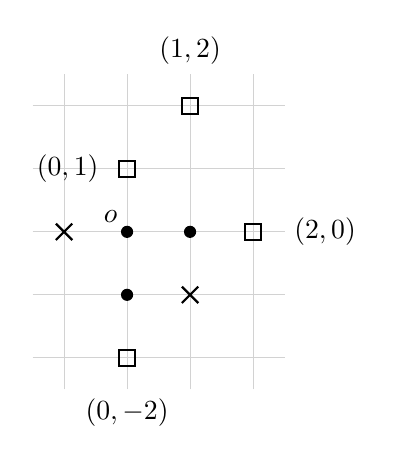
\begin{tikzpicture}[x=8mm,y=8mm]
\draw[gray!35,step=1] (-1.5,-2.5) grid (2.5,2.5);
\foreach \x/\y in {0/0,1/0,0/-1}{\fill (\x,\y) circle (2.2pt);}
\foreach \x/\y in {1/-1,-1/0}{
 \draw[thick] (\x-.13,\y-.13)--(\x+.13,\y+.13)
              (\x-.13,\y+.13)--(\x+.13,\y-.13);}
\foreach \x/\y in {0/1,0/-2,2/0,1/2}{
 \draw[thick] (\x-.13,\y-.13) rectangle (\x+.13,\y+.13);}
\node[above left] at (0,0) {$o$};
\node[right] at (2.5,0) {$(2,0)$};
\node[left] at (-.3,1) {$(0,1)$};
\node[above] at (1,2.5) {$(1,2)$};
\node[below] at (0,-2.5) {$(0,-2)$};
\end{tikzpicture}
\caption{After the exceptional reply \((-1,0)\) and Maker's claim
\((0,-1)\), the filled dots form \(Q\) and the crosses are the two
Breaker cells.  Hollow squares mark possible pivots after Breaker's
next reply.  The diagram displays their geometry; their availability
is determined by the seven envelopes specified by the terms in
Table~\ref{r35:exception-children}.}
\label{r35:bent-figure}
\end{figure}

\section{Exact scope of the finite reconstruction supplement}
\label{app:formal}\label{rformal:main}

This appendix records the scope of the finite reconstruction supplement
for the 35-move certificate.  The conventional proofs in this article
are independent of this supplement.

\subsection{The finite reconstruction theorem}
\label{rformal:evidence}

The finite reconstruction supplement linked from
\path{../../lean/docs/187.md}, relative to the
article root, has the endpoint
\texttt{OAI.SnakyCertificate.certificate\_correct}.  Its definitions fix
the target, six ordered base points, eight letter-order orientations,
offset-by-four translation digits, and full-envelope recurrence of
Appendix~\ref{app:route35}.  The formal envelope symbol $H$ denotes
$T_i^{35}$ in that appendix.  The theorem has seven clauses:
\begin{enumerate}
\item The table has exactly 610 nonbase rows, indexed $6$ through
$615$, each with a nonempty list of allowed placements referencing
earlier rows.
\item There are exactly 1,837 ordered placement terms, counted with
multiplicity.
\item Row $557$ has required set $\{(-1,0)\}$, envelope size $118$,
height $19$, and no envelope cell with $x\leq-3$ and $y\leq-2$.
\item Row $595$ has required set $\{(-1,0)\}$, envelope size $222$,
height $27$, and no envelope cell with $x=-2$ and $y\leq-2$.
\item Row $603$ has required set $\{(-1,0)\}$, envelope size $275$,
height $27$, and no envelope cell with $x\leq-3$ and $y=0$.
\item Row $615$ has required set $\{(1,0)\}$, envelope size $686$,
height $34$, and omits $(1,-1)$ from its envelope.
\item Every row $0$ through $615$ satisfies
$A_i^{35}\subseteq T_i^{35}$,
$(0,0)\in T_i^{35}\setminus A_i^{35}$, and $h_i^{35}\leq34$.
\end{enumerate}
The last clause makes the required-set containment proper.  The
literal entries in the Lean source agree with the printed
letter-and-offset certificate.  This is a finite reconstruction
statement, not a game-winning theorem: it does not include the opening,
the arbitrary-ownership and Breaker-turn interfaces, policy extraction,
or the additional tactical conclusions of Appendix~\ref{app:route35}.
The conventional arguments supply these game-theoretic implications.

The finite Python reconstructions described in this article are separate
from Lean kernel checking; they do not themselves establish a Lean theorem
or kernel compilation.  The certificate copy under
\path{verification/supporting/prior-35/} contains only the literal certificate data.

\section{Complete certificate data}\label{app:data}

The following listing contains every line of the certificate used
in Proposition~\ref{prop:certificate}, without omissions.
Cards $0,\ldots,5$ are the six bases \eqref{eq:bases}; the listing
starts at card $6$. The grammar and bit-coded placements are
specified in Section~\ref{sec:certificate}.
A long logical line may wrap visually. The editable file
\texttt{verification/certificate.txt} has one logical line per numbered card.
Parentheses describe inline applications of exactly the same
combination rule, with coordinates in the enclosing line's frame.

\lstinputlisting[breakatwhitespace=true,frame=single]{../verification/certificate.txt}

\section{Complete reduced-envelope certificate}\label{app:data25}

This is the complete decimal certificate of Appendix~\ref{app:route25}.
It begins at card $6$ and ends at card $2015$, after the six bases
specified there. A marker beginning with \texttt{\#} states the next
card number; it is not itself a card. Each other nonempty logical line
is one composition. Every three-digit block, including its leading
zeros, belongs to the decimal grammar. For readable line breaking,
the displayed numeric rows have a bracketed card number and spaces
between blocks. Remove that bracketed prefix and those spaces to
recover each exact numeric line of the literal file; markers and blank
lines are unchanged. This reversible formatting is checked in the
source distribution. Long rows may wrap visually.

\lstinputlisting[breakatwhitespace=true,frame=single]{../verification/supporting/route25/certificate-display.txt}

\section{Complete letter-and-offset certificate}\label{app:data35}

This listing supplies every row $6$ through $615$ of the $35$-move
certificate. Appendix~\ref{app:route35} defines the six base cards,
every letter and translation offset, and the complete reconstruction.
Each line starts with its row number, followed by a nonempty list of
placed earlier cards. Long logical lines may wrap visually.

\lstinputlisting[breakatwhitespace=true,frame=single]{../verification/supporting/prior-35/certificate.txt}

\section{Complete executable verifier}\label{app:checker}

The verifier below reads the literal certificate and evaluates the
set operations described in the paper. From the paper root,
run
\begin{lstlisting}[basicstyle=\ttfamily\small]
python3 verification/verify_certificate.py
\end{lstlisting}
An explicit input path may be supplied with \texttt{--table}.
The wrapper rejects any data bytes with a different checksum and
refuses optimized Python execution, which would disable the
assertions in the checking function. Successful termination means
that every executed check has passed; the semantic implication is
the induction in Proposition~\ref{prop:certificate} and
Lemma~\ref{lem:combination}.

The arrays \texttt{AA}, \texttt{TT}, and \texttt{HH} hold the required
sets, envelopes, and heights of completed numbered cards.
The recursive function \texttt{expr} evaluates an inline expression
in the current line's coordinate frame. A reference uses an earlier
array entry; it never interprets an inline pivot as a translation.
All computations use exact Python integers and finite sets.

\begingroup
\fontencoding{T1}\selectfont
\renewcommand{\ttdefault}{lmtt}
\lstinputlisting[language=Python,breakatwhitespace=false,
 frame=single]{../verification/verify_certificate.py}
\endgroup

\subsection{Independent reconstructions of all three certificates}

The source distribution contains an additional, independently parsed
reconstruction for every dialect, together with tests of the finite
identities used in the article. From the paper root run
\begin{lstlisting}[basicstyle=\ttfamily\small]
python3 verification/supporting/verify_all.py --output-dir ../all-checks
\end{lstlisting}
Choose a new output directory outside the paper directory. The command
runs the primary and independent checks for all three literal tables
and records their full-card agreement, exact identities, and rejection
tests. The support guide gives each program's standalone command.
The $21$-move programs under \texttt{verification/supporting/route21/} additionally
check every inline node and local reply class; they are distinct from
the short verifier printed above. The $25$-move programs under
\texttt{verification/supporting/route25/} use the reduced sets and swap-first anchor
maps. The programs under \texttt{verification/supporting/route35/} check the
letter-and-offset table and its conditional and tactical identities.
All three literal tables and every checking program are included in
the editable source distribution. The directory
\texttt{verification/supporting/prior-35/} contains only a copy of the $35$-move
literal certificate. The scope of the finite reconstruction supplement
is stated in Appendix~\ref{app:formal}.

\end{document}
